\chapter{Actuators in Real Control Systems}
\label{ch:actuators}

\whythismatters{
Every control system needs something that can actually \textit{do} work---an actuator that converts control signals into physical action. When you command a robot arm to move, electric motors spin. When an aircraft adjusts its flight path, hydraulic cylinders push control surfaces. When a chemical process needs more heat, valves open to admit steam. Understanding actuator dynamics is not optional for control engineers; it's fundamental. A controller designed assuming instantaneous, unlimited actuation will fail when it encounters the bandwidth limits, saturation, and nonlinearities of real actuators. In this chapter, we develop comprehensive models for the actuators you'll encounter throughout your career: DC motors, servo systems, hydraulic cylinders, and pneumatic actuators. We derive transfer functions from first principles, analyze practical limitations, and work through detailed examples that bridge theory and application.
}

\section{Introduction to Actuator Dynamics}

In the previous chapter, we developed systematic techniques for modeling physical systems and linearizing nonlinear dynamics around operating points. Those techniques gave us mathematical models that describe how systems respond to inputs. But what generates those inputs? In any feedback control system, the answer is \textit{actuators}---the components that convert control signals into physical forces, torques, flows, or displacements.

The actuator is where control theory meets physical reality. Your beautifully designed controller produces a command signal, perhaps a voltage or a digital value. The actuator must translate that signal into mechanical work, and this translation process has its own dynamics, limitations, and nonlinearities. Ignoring actuator dynamics is one of the most common mistakes made by novice control engineers, and it leads to controllers that work perfectly in simulation but fail on real hardware.

\subsection{Why Actuator Modeling Matters}

Consider what happens when you design a position controller for a robotic joint. You might model the joint as a simple inertia with some damping, design a PID controller with nice phase margins, and simulate beautiful step responses. But when you implement this controller on actual hardware, you discover:

\begin{itemize}
    \item The motor can't change current instantaneously---there's an electrical time constant
    \item The motor driver saturates at some maximum voltage and current
    \item There's backlash in the gearbox that creates position-dependent dead zones
    \item Friction in the bearings creates stick-slip behavior at low speeds
    \item The motor heats up during operation, changing its resistance and torque constant
\end{itemize}

Each of these effects can destabilize your carefully designed controller or dramatically degrade its performance. The solution is to model these effects explicitly and either design the controller to accommodate them or add compensation strategies.

\subsection{Actuator Categories}

We'll study three major categories of actuators in this chapter:

\textbf{Electromagnetic Actuators:} These convert electrical energy to mechanical motion through magnetic fields. DC motors (both brushed and brushless) are the workhorses of motion control, found in everything from computer disk drives to electric vehicles. We'll develop detailed models including electrical dynamics, back-EMF coupling, friction, and thermal effects.

\textbf{Hydraulic Actuators:} These use pressurized fluid to generate very high forces in compact packages. Hydraulic systems dominate in heavy machinery, aircraft control surfaces, and industrial presses. Their dynamics involve fluid compressibility, valve characteristics, and complex friction behavior.

\textbf{Pneumatic Actuators:} These use compressed gas, typically air, as the working fluid. While similar to hydraulics in some ways, the high compressibility of gases creates fundamentally different dynamics that require special treatment.

\subsection{Common Actuator Characteristics}

Despite their physical differences, all actuators share certain characteristics that affect control design:

\begin{enumerate}
    \item \textbf{Bandwidth:} Every actuator has limited speed of response. Motors can't change torque instantaneously due to electrical inductance. Hydraulic valves have finite slew rates. This bandwidth limitation constrains how fast your controller can be.

    \item \textbf{Saturation:} Real actuators have maximum outputs. Motors have maximum torque (limited by current capacity and thermal constraints). Hydraulic cylinders have maximum force (limited by supply pressure). Controllers must be designed to handle saturation gracefully.

    \item \textbf{Dead Zones:} Many actuators don't respond to small inputs. Friction prevents motion until sufficient force is applied. Valves may have overlap regions where small movements produce no flow. These create challenges for precision control.

    \item \textbf{Nonlinearities:} The relationship between input and output is rarely perfectly linear. Back-EMF in motors creates speed-dependent effects. Orifice flow in hydraulics is proportional to the square root of pressure. Careful modeling of these nonlinearities is essential.

    \item \textbf{Coupling:} Actuator behavior often depends on the load. A motor's speed affects its back-EMF, which affects its current, which affects its torque. Hydraulic cylinder pressure depends on load force. These couplings must be captured in our models.
\end{enumerate}

In the sections that follow, we'll develop detailed models for each actuator type, derive transfer functions suitable for control design, and examine the practical limitations that affect real-world performance.

%===============================================================================
\section{DC Motor Fundamentals}
\label{sec:dc_motor_fundamentals}
%===============================================================================

The DC motor is perhaps the most important actuator in control systems education and practice. Its relatively simple physics leads to tractable mathematical models, yet it exhibits all the key phenomena---electrical dynamics, electromechanical coupling, friction, saturation---that characterize more complex actuators. Understanding DC motors thoroughly prepares you for studying any electromagnetic actuator.

\subsection{Basic Operating Principles}

A DC motor converts electrical energy to mechanical rotational energy through electromagnetic induction. The fundamental physics relies on two laws:

\textbf{Lorentz Force Law:} A current-carrying conductor in a magnetic field experiences a force perpendicular to both the current direction and the magnetic field:
\begin{equation}
    \mathbf{F} = I \mathbf{L} \times \mathbf{B}
\end{equation}
where $I$ is the current, $\mathbf{L}$ is the conductor length vector, and $\mathbf{B}$ is the magnetic flux density. This force creates the torque that spins the motor.

\textbf{Faraday's Law of Induction:} A conductor moving through a magnetic field has an induced voltage (electromotive force) proportional to the rate of change of magnetic flux:
\begin{equation}
    e = -\frac{d\Phi}{dt}
\end{equation}
For a rotating motor, this creates a voltage proportional to angular velocity, called the \textit{back-EMF}.

These two laws create a fundamental coupling between electrical and mechanical domains: current produces torque (motor action), and motion produces voltage (generator action). This coupling is the key to understanding DC motor dynamics.

\subsection{Motor Construction}

A typical brushed DC motor consists of:

\begin{itemize}
    \item \textbf{Stator:} The stationary outer part containing permanent magnets or field windings that create the magnetic field
    \item \textbf{Rotor (Armature):} The rotating inner part with windings that carry the armature current
    \item \textbf{Commutator:} A mechanical switch that reverses the current direction in the armature windings as the rotor turns, maintaining unidirectional torque
    \item \textbf{Brushes:} Spring-loaded contacts that transfer current from the external circuit to the rotating commutator
\end{itemize}

The commutator and brushes are the characteristic feature of brushed DC motors. They automatically switch the current direction to maintain continuous rotation, but they also introduce friction, wear, and electrical noise. Brushless DC motors eliminate these components by using electronic commutation, which we'll discuss later.

\subsection{Torque Generation}

The electromagnetic torque generated by a DC motor is proportional to two quantities: the magnetic flux in the air gap and the armature current. For a motor with constant field (either permanent magnets or separately excited field windings), this relationship is remarkably simple:

\begin{equation}
    \boxed{T_e = K_t I_a}
    \label{eq:torque_constant}
\end{equation}

where:
\begin{itemize}
    \item $T_e$ = electromagnetic torque (N$\cdot$m)
    \item $K_t$ = torque constant (N$\cdot$m/A)
    \item $I_a$ = armature current (A)
\end{itemize}

The torque constant $K_t$ depends on motor construction: the number of armature conductors, the number of pole pairs, and the magnetic flux density in the air gap. For a given motor, $K_t$ is essentially constant (until magnetic saturation occurs at very high currents).

\keypoint{The linear relationship between torque and current, $T_e = K_t I_a$, is one of the most important properties of DC motors for control. It means we can control torque directly by controlling current---no complex inverse models required.}

\subsection{Back-EMF (Counter Electromotive Force)}

When the motor rotates, the armature conductors move through the magnetic field, inducing a voltage that opposes the applied voltage. This is the \textit{back-EMF} (sometimes called counter-EMF):

\begin{equation}
    \boxed{E_b = K_e \omega}
    \label{eq:back_emf}
\end{equation}

where:
\begin{itemize}
    \item $E_b$ = back-EMF voltage (V)
    \item $K_e$ = back-EMF constant (V$\cdot$s/rad)
    \item $\omega$ = angular velocity (rad/s)
\end{itemize}

The back-EMF constant $K_e$ depends on the same motor construction parameters as $K_t$. In fact, for a DC motor with consistent units, these constants are numerically equal:

\begin{equation}
    \boxed{K_t \text{ (N$\cdot$m/A)} = K_e \text{ (V$\cdot$s/rad)}}
    \label{eq:kt_ke_equality}
\end{equation}

This equality is a direct consequence of energy conservation in the electromechanical conversion process. We can prove it as follows:

\textbf{Proof:} The electrical power converted to mechanical power is:
\begin{equation}
    P_{em} = E_b I_a = K_e \omega I_a
\end{equation}

The mechanical power produced is:
\begin{equation}
    P_{mech} = T_e \omega = K_t I_a \omega
\end{equation}

For energy conservation, $P_{em} = P_{mech}$, which requires $K_e = K_t$. $\square$

\warningbox{The equality $K_t = K_e$ holds only when both constants are expressed in consistent SI units. Motor datasheets often give $K_e$ in V/krpm, which must be converted to V$\cdot$s/rad for this equality to hold. The conversion is: $K_e$ (V$\cdot$s/rad) $= K_e$ (V/krpm) $\times \frac{1000}{60} \times \frac{1}{2\pi} = K_e$ (V/krpm) $\times$ 0.1047.}

\subsection{Electrical Dynamics}

The armature circuit can be modeled as a resistor $R_a$ and inductor $L_a$ in series with the back-EMF source. Applying Kirchhoff's voltage law:

\begin{equation}
    V_a = R_a I_a + L_a \frac{dI_a}{dt} + E_b
    \label{eq:electrical_kvl}
\end{equation}

where $V_a$ is the applied armature voltage.

Substituting the back-EMF expression:
\begin{equation}
    \boxed{V_a = R_a I_a + L_a \frac{dI_a}{dt} + K_e \omega}
    \label{eq:electrical_equation}
\end{equation}

This is the \textbf{electrical equation} of the DC motor. It shows how the armature current depends on both the applied voltage and the motor speed (through back-EMF).

\textbf{Physical Interpretation:} When voltage is first applied to a stationary motor, there's no back-EMF, so current rises rapidly (limited only by inductance). As the motor accelerates, back-EMF increases, which opposes current flow, causing current to decrease until a balance is reached. At steady state with no load, the back-EMF nearly equals the applied voltage, and only a small current flows to overcome friction.

\subsection{Mechanical Dynamics}

The mechanical side of the motor is governed by Newton's second law for rotation:

\begin{equation}
    J \frac{d\omega}{dt} = T_e - T_f - T_L
    \label{eq:mechanical_newton}
\end{equation}

where:
\begin{itemize}
    \item $J$ = total moment of inertia (kg$\cdot$m$^2$), including rotor and any coupled load
    \item $T_e = K_t I_a$ = electromagnetic torque
    \item $T_f$ = friction torque
    \item $T_L$ = load torque (external load)
\end{itemize}

For initial analysis, we often model friction as purely viscous:
\begin{equation}
    T_f = b \omega
\end{equation}
where $b$ is the viscous friction coefficient (N$\cdot$m$\cdot$s/rad).

Substituting:
\begin{equation}
    \boxed{J \frac{d\omega}{dt} = K_t I_a - b \omega - T_L}
    \label{eq:mechanical_equation}
\end{equation}

This is the \textbf{mechanical equation} of the DC motor.

\subsection{Complete Dynamic Model}

Combining the electrical and mechanical equations, we have a complete description of DC motor dynamics:

\begin{empheq}[box=\fbox]{align}
    L_a \frac{dI_a}{dt} &= V_a - R_a I_a - K_e \omega \label{eq:motor_electrical}\\
    J \frac{d\omega}{dt} &= K_t I_a - b \omega - T_L \label{eq:motor_mechanical}
\end{empheq}

These two coupled first-order differential equations describe how armature current and angular velocity evolve over time in response to applied voltage $V_a$ and load torque $T_L$.

The coupling between equations is crucial:
\begin{itemize}
    \item Current $I_a$ appears in the mechanical equation (torque generation)
    \item Velocity $\omega$ appears in the electrical equation (back-EMF)
\end{itemize}

This coupling creates the characteristic behavior of DC motors: applying voltage causes current to flow, which creates torque, which causes acceleration, which increases back-EMF, which reduces current, until equilibrium is reached.

\subsection{Electrical and Mechanical Time Constants}

The DC motor has two characteristic time constants that govern its dynamics:

\textbf{Electrical Time Constant:}
\begin{equation}
    \boxed{\tau_e = \frac{L_a}{R_a}}
    \label{eq:electrical_time_constant}
\end{equation}

This governs how quickly the armature current responds to voltage changes (with the rotor held stationary, so back-EMF is constant). Physically, it's the time for current to reach 63.2\% of its final value after a step voltage input.

\textbf{Typical values:}
\begin{itemize}
    \item Small DC motors ($<$ 100 W): 0.5--5 ms
    \item Medium motors (100 W--1 kW): 2--20 ms
    \item Large motors ($>$ 1 kW): 10--50 ms
\end{itemize}

\textbf{Mechanical Time Constant:}
\begin{equation}
    \boxed{\tau_m = \frac{R_a J}{K_t K_e} = \frac{R_a J}{K_t^2}}
    \label{eq:mechanical_time_constant}
\end{equation}

This governs how quickly the motor speed responds to torque changes (neglecting electrical dynamics). Physically, it's the time for an unloaded motor to reach 63.2\% of its no-load speed after applying rated voltage.

\textbf{Typical values:}
\begin{itemize}
    \item Small servo motors: 5--50 ms
    \item Medium industrial motors: 50--200 ms
    \item Large motors with high inertia: 200--1000 ms
\end{itemize}

\keypoint{For most DC motors, $\tau_e \ll \tau_m$---the electrical dynamics are much faster than the mechanical dynamics. This means the current settles to its quasi-steady-state value quickly compared to how fast the motor accelerates. This separation of time scales often allows us to neglect electrical dynamics in speed control applications, treating current response as instantaneous.}

\subsection{Torque-Speed Characteristics}

One of the most useful properties of DC motors is their linear torque-speed characteristic. Starting from the steady-state electrical equation (with $dI_a/dt = 0$):

\begin{equation}
    V_a = R_a I_a + K_e \omega
\end{equation}

Solving for current:
\begin{equation}
    I_a = \frac{V_a - K_e \omega}{R_a}
\end{equation}

Substituting into the torque equation:
\begin{equation}
    T_e = K_t I_a = K_t \frac{V_a - K_e \omega}{R_a} = \frac{K_t}{R_a} V_a - \frac{K_t K_e}{R_a} \omega
\end{equation}

Since $K_t = K_e$:
\begin{equation}
    \boxed{T_e = \frac{K_t}{R_a} V_a - \frac{K_t^2}{R_a} \omega}
    \label{eq:torque_speed}
\end{equation}

This is a \textbf{linear relationship} between torque and speed! At any given voltage, the motor's operating point lies on a straight line in the torque-speed plane.

\textbf{Key Operating Points:}

\textit{Stall Torque} (when $\omega = 0$):
\begin{equation}
    T_{stall} = \frac{K_t V_a}{R_a}
\end{equation}

\textit{No-Load Speed} (when $T_e = 0$):
\begin{equation}
    \omega_{no-load} = \frac{V_a}{K_e}
\end{equation}

The torque-speed line connects these two points:
\begin{equation}
    T_e = T_{stall} \left(1 - \frac{\omega}{\omega_{no-load}}\right)
\end{equation}

\textbf{Maximum Power Point:}

The mechanical output power is $P = T_e \omega$. Substituting the torque-speed relationship:
\begin{equation}
    P = T_{stall} \omega - \frac{T_{stall}}{\omega_{no-load}} \omega^2
\end{equation}

Taking the derivative and setting to zero:
\begin{equation}
    \frac{dP}{d\omega} = T_{stall} - \frac{2 T_{stall}}{\omega_{no-load}} \omega = 0
\end{equation}

Solving:
\begin{equation}
    \omega_{max-power} = \frac{\omega_{no-load}}{2}, \quad T_{max-power} = \frac{T_{stall}}{2}
\end{equation}

\begin{equation}
    \boxed{P_{max} = \frac{T_{stall} \cdot \omega_{no-load}}{4}}
\end{equation}

Maximum power occurs at exactly half the no-load speed and half the stall torque.

\warningbox{Operating at or near stall torque is dangerous for most motors. With no rotation to provide cooling airflow and maximum current flowing, the motor heats rapidly. Stall conditions should be momentary only. Continuous operation is typically limited to 20--50\% of stall torque depending on motor design and cooling.}

%===============================================================================
\section{Motor Dynamics and Transfer Functions}
\label{sec:motor_transfer_functions}
%===============================================================================

Having established the governing equations, we now derive transfer functions that relate motor inputs to outputs. These transfer functions are essential for control system design and analysis.

\subsection{State-Space Representation}

The natural state variables for a DC motor are armature current $I_a$ and angular velocity $\omega$. From our dynamic equations \eqref{eq:motor_electrical} and \eqref{eq:motor_mechanical}:

\begin{equation}
    \begin{aligned}
        \frac{dI_a}{dt} &= -\frac{R_a}{L_a} I_a - \frac{K_e}{L_a} \omega + \frac{1}{L_a} V_a \\
        \frac{d\omega}{dt} &= \frac{K_t}{J} I_a - \frac{b}{J} \omega - \frac{1}{J} T_L
    \end{aligned}
\end{equation}

In state-space form with state vector $\mathbf{x} = [I_a, \omega]^T$:

\begin{equation}
    \boxed{
    \dot{\mathbf{x}} = \begin{bmatrix} -\frac{R_a}{L_a} & -\frac{K_e}{L_a} \\[6pt] \frac{K_t}{J} & -\frac{b}{J} \end{bmatrix} \mathbf{x} + \begin{bmatrix} \frac{1}{L_a} & 0 \\[6pt] 0 & -\frac{1}{J} \end{bmatrix} \begin{bmatrix} V_a \\ T_L \end{bmatrix}
    }
    \label{eq:motor_state_space}
\end{equation}

Or more compactly:
\begin{equation}
    \dot{\mathbf{x}} = \mathbf{A} \mathbf{x} + \mathbf{B} \mathbf{u}
\end{equation}

with:
\begin{equation}
    \mathbf{A} = \begin{bmatrix} -\frac{R_a}{L_a} & -\frac{K_e}{L_a} \\[6pt] \frac{K_t}{J} & -\frac{b}{J} \end{bmatrix}, \quad
    \mathbf{B} = \begin{bmatrix} \frac{1}{L_a} & 0 \\[6pt] 0 & -\frac{1}{J} \end{bmatrix}, \quad
    \mathbf{u} = \begin{bmatrix} V_a \\ T_L \end{bmatrix}
\end{equation}

If we measure angular velocity as output:
\begin{equation}
    y = \omega = \begin{bmatrix} 0 & 1 \end{bmatrix} \mathbf{x}
\end{equation}

so $\mathbf{C} = [0 \; 1]$ and $\mathbf{D} = [0 \; 0]$.

\subsection{Transfer Function: Voltage to Speed (Full Model)}

To derive the transfer function from voltage to speed, we take Laplace transforms of the governing equations (assuming zero initial conditions and setting $T_L = 0$ for now):

\textbf{Electrical:}
\begin{equation}
    V_a(s) = (R_a + L_a s) I_a(s) + K_e \Omega(s)
    \label{eq:laplace_electrical}
\end{equation}

\textbf{Mechanical:}
\begin{equation}
    K_t I_a(s) = (Js + b) \Omega(s)
    \label{eq:laplace_mechanical}
\end{equation}

From the mechanical equation:
\begin{equation}
    I_a(s) = \frac{(Js + b)}{K_t} \Omega(s)
\end{equation}

Substituting into the electrical equation:
\begin{equation}
    V_a(s) = (R_a + L_a s) \frac{(Js + b)}{K_t} \Omega(s) + K_e \Omega(s)
\end{equation}

\begin{equation}
    V_a(s) = \left[ \frac{(R_a + L_a s)(Js + b)}{K_t} + K_e \right] \Omega(s)
\end{equation}

Solving for the transfer function:
\begin{equation}
    G_\omega(s) = \frac{\Omega(s)}{V_a(s)} = \frac{K_t}{(R_a + L_a s)(Js + b) + K_t K_e}
\end{equation}

Expanding the denominator:
\begin{equation}
    (R_a + L_a s)(Js + b) + K_t K_e = L_a J s^2 + (L_a b + R_a J) s + (R_a b + K_t K_e)
\end{equation}

\begin{equation}
    \boxed{G_\omega(s) = \frac{\Omega(s)}{V_a(s)} = \frac{K_t}{L_a J s^2 + (L_a b + R_a J) s + (R_a b + K_t K_e)}}
    \label{eq:motor_tf_full}
\end{equation}

This is a \textbf{second-order transfer function}. The two poles correspond to the coupled electrical and mechanical dynamics.

\textbf{DC Gain:} Setting $s = 0$:
\begin{equation}
    G_\omega(0) = \frac{K_t}{R_a b + K_t K_e}
\end{equation}

If viscous friction $b$ is small compared to electromagnetic damping:
\begin{equation}
    G_\omega(0) \approx \frac{K_t}{K_t K_e} = \frac{1}{K_e}
\end{equation}

This makes physical sense: at steady state with no friction, the speed is determined by voltage divided by back-EMF constant.

\subsection{Simplified First-Order Model}

When the electrical time constant is much smaller than the mechanical time constant ($\tau_e \ll \tau_m$), we can neglect electrical dynamics. Setting $L_a = 0$ in the full transfer function:

\begin{equation}
    G_\omega(s) \approx \frac{K_t}{R_a J s + (R_a b + K_t K_e)}
\end{equation}

Factoring:
\begin{equation}
    G_\omega(s) = \frac{K_t/(R_a b + K_t K_e)}{1 + \frac{R_a J}{R_a b + K_t K_e} s}
\end{equation}

If $R_a b \ll K_t K_e$ (electromagnetic damping dominates viscous friction):

\begin{equation}
    \boxed{G_\omega(s) \approx \frac{1/K_e}{1 + \tau_m s} = \frac{K_{dc}}{1 + \tau_m s}}
    \label{eq:motor_tf_simplified}
\end{equation}

where:
\begin{itemize}
    \item $K_{dc} = 1/K_e$ = DC gain (rad/s per volt)
    \item $\tau_m = R_a J / K_t^2$ = mechanical time constant
\end{itemize}

This first-order model is remarkably useful for speed control design. It captures the essential dynamics while being simple enough for straightforward controller synthesis.

\keypoint{The simplified first-order model $G(s) = K_{dc}/(1 + \tau_m s)$ is valid when: (1) electrical dynamics are fast compared to mechanical ($\tau_e \ll \tau_m$), and (2) electromagnetic damping dominates viscous friction ($K_t K_e \gg R_a b$). These conditions hold for most small to medium DC motors.}

\subsection{Transfer Function: Voltage to Position}

For position control, we need position $\theta$ as output. Since $\theta = \int \omega \, dt$, in the Laplace domain:
\begin{equation}
    \Theta(s) = \frac{\Omega(s)}{s}
\end{equation}

Therefore:
\begin{equation}
    G_\theta(s) = \frac{\Theta(s)}{V_a(s)} = \frac{G_\omega(s)}{s}
\end{equation}

Using the full model:
\begin{equation}
    \boxed{G_\theta(s) = \frac{K_t}{s[L_a J s^2 + (L_a b + R_a J) s + (R_a b + K_t K_e)]}}
    \label{eq:motor_tf_position_full}
\end{equation}

Using the simplified model:
\begin{equation}
    \boxed{G_\theta(s) = \frac{K_{dc}}{s(1 + \tau_m s)} = \frac{1/K_e}{s(1 + \tau_m s)}}
    \label{eq:motor_tf_position_simplified}
\end{equation}

The position transfer function has an integrator ($1/s$), making it a \textbf{Type 1 system}. This has important implications for control: the motor naturally integrates velocity to produce position, which helps with steady-state tracking but requires careful stabilization.

\subsection{Transfer Function: Load Torque to Speed}

Load torque $T_L$ acts as a disturbance. The transfer function from $T_L$ to $\Omega$ (with $V_a = 0$) describes how well the motor rejects load disturbances.

From the Laplace equations with $V_a = 0$:
\begin{equation}
    0 = (R_a + L_a s) I_a(s) + K_e \Omega(s)
\end{equation}
\begin{equation}
    K_t I_a(s) - T_L(s) = (Js + b) \Omega(s)
\end{equation}

From the first equation: $I_a(s) = -\frac{K_e}{R_a + L_a s} \Omega(s)$

Substituting into the second:
\begin{equation}
    -\frac{K_t K_e}{R_a + L_a s} \Omega(s) - T_L(s) = (Js + b) \Omega(s)
\end{equation}

Solving:
\begin{equation}
    \boxed{G_d(s) = \frac{\Omega(s)}{T_L(s)} = \frac{-(R_a + L_a s)}{L_a J s^2 + (L_a b + R_a J) s + (R_a b + K_t K_e)}}
    \label{eq:motor_tf_disturbance}
\end{equation}

The negative sign indicates that positive load torque (opposing motion) reduces speed, as expected.

Using the simplified model ($L_a = 0$):
\begin{equation}
    G_d(s) \approx \frac{-R_a}{R_a J s + (R_a b + K_t K_e)} = \frac{-R_a/(R_a b + K_t K_e)}{1 + \tau_m s}
\end{equation}

\textbf{Steady-State Speed Droop:} The DC gain of the disturbance transfer function gives the steady-state speed change per unit load torque:
\begin{equation}
    \frac{\Delta \omega}{\Delta T_L}\bigg|_{ss} = G_d(0) = \frac{-R_a}{R_a b + K_t K_e} \approx \frac{-R_a}{K_t^2}
\end{equation}

This is the motor's \textit{regulation} or \textit{speed droop}---how much speed drops when load increases. A motor with higher $K_t$ (more torque per amp) has better regulation.

\subsection{State-Space for Position Control}

For position control, we add position as a third state variable: $\mathbf{x} = [I_a, \omega, \theta]^T$

\begin{equation}
    \dot{\mathbf{x}} = \begin{bmatrix} -\frac{R_a}{L_a} & -\frac{K_e}{L_a} & 0 \\[6pt] \frac{K_t}{J} & -\frac{b}{J} & 0 \\[6pt] 0 & 1 & 0 \end{bmatrix} \mathbf{x} + \begin{bmatrix} \frac{1}{L_a} \\[6pt] 0 \\[6pt] 0 \end{bmatrix} V_a + \begin{bmatrix} 0 \\[6pt] -\frac{1}{J} \\[6pt] 0 \end{bmatrix} T_L
    \label{eq:motor_state_space_position}
\end{equation}

The third row simply states $\dot{\theta} = \omega$.

%===============================================================================
\section{Motor Drives and Power Electronics}
\label{sec:motor_drives}
%===============================================================================

A DC motor cannot be driven directly from a control computer's output. Between the controller and motor sits the \textit{motor drive}---power electronics that amplify control signals to levels capable of driving significant current through the motor windings. Understanding drive dynamics is essential because they introduce their own bandwidth limitations, nonlinearities, and constraints.

\subsection{The H-Bridge: Bidirectional Motor Control}

The fundamental building block of DC motor drives is the \textbf{H-bridge}---a circuit that allows voltage to be applied across a load in either direction. The name comes from the schematic shape, which resembles the letter H.

An H-bridge consists of four switching devices (typically MOSFETs or IGBTs) arranged in two ``legs,'' with the motor connected between the midpoints:

\begin{center}
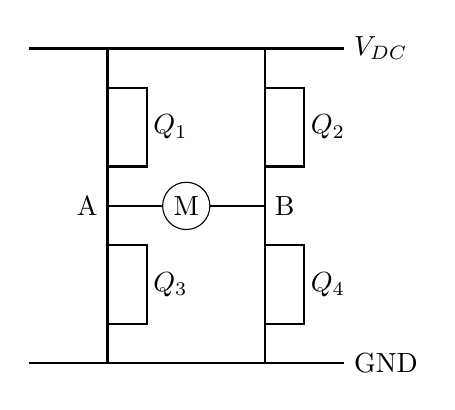
\begin{tikzpicture}[scale=1.0]
    % Power rails
    \draw[thick] (-2,2) -- (2,2) node[right] {$V_{DC}$};
    \draw[thick] (-2,-2) -- (2,-2) node[right] {GND};

    % Left leg
    \draw[thick] (-1,2) -- (-1,1.5);
    \draw[thick] (-1,1.5) -- (-0.5,1.5) -- (-0.5,0.5) -- (-1,0.5) -- (-1,1.5);
    \node at (-0.2,1) {$Q_1$};
    \draw[thick] (-1,0.5) -- (-1,0);

    \draw[thick] (-1,0) -- (-1,-0.5);
    \draw[thick] (-1,-0.5) -- (-0.5,-0.5) -- (-0.5,-1.5) -- (-1,-1.5) -- (-1,-0.5);
    \node at (-0.2,-1) {$Q_3$};
    \draw[thick] (-1,-1.5) -- (-1,-2);

    % Right leg
    \draw[thick] (1,2) -- (1,1.5);
    \draw[thick] (1,1.5) -- (1.5,1.5) -- (1.5,0.5) -- (1,0.5) -- (1,1.5);
    \node at (1.8,1) {$Q_2$};
    \draw[thick] (1,0.5) -- (1,0);

    \draw[thick] (1,0) -- (1,-0.5);
    \draw[thick] (1,-0.5) -- (1.5,-0.5) -- (1.5,-1.5) -- (1,-1.5) -- (1,-0.5);
    \node at (1.8,-1) {$Q_4$};
    \draw[thick] (1,-1.5) -- (1,-2);

    % Motor
    \draw[thick] (-1,0) -- (-0.3,0);
    \draw[thick] (0.3,0) -- (1,0);
    \draw (0,0) circle (0.3);
    \node at (0,0) {M};

    % Labels
    \node at (-1,0) [left] {A};
    \node at (1,0) [right] {B};
\end{tikzpicture}
\end{center}

\textbf{Operating Modes:}

\begin{itemize}
    \item \textbf{Forward:} $Q_1$ and $Q_4$ ON, $Q_2$ and $Q_3$ OFF $\Rightarrow$ Current flows A to B, motor turns one direction
    \item \textbf{Reverse:} $Q_2$ and $Q_3$ ON, $Q_1$ and $Q_4$ OFF $\Rightarrow$ Current flows B to A, motor turns opposite direction
    \item \textbf{Brake (Low-side):} $Q_3$ and $Q_4$ ON, $Q_1$ and $Q_2$ OFF $\Rightarrow$ Motor terminals shorted through ground, dynamic braking
    \item \textbf{Coast:} All switches OFF $\Rightarrow$ Motor terminals open, motor coasts with back-EMF driving current through body diodes
\end{itemize}

\warningbox{Never turn on both switches in the same leg simultaneously ($Q_1$ and $Q_3$, or $Q_2$ and $Q_4$). This creates a direct short from $V_{DC}$ to ground---a ``shoot-through'' condition that can destroy the switches instantly. H-bridge drivers must include dead-time logic to prevent this.}

\subsection{Pulse Width Modulation (PWM)}

Rather than varying voltage continuously (which would require inefficient linear amplifiers), motor drives use \textbf{Pulse Width Modulation (PWM)}. The switches are turned fully ON or fully OFF, but the duty cycle (fraction of time ON) is varied to control average voltage.

\textbf{PWM Fundamentals:}

For a PWM signal with period $T$ and ON-time $t_{on}$:
\begin{equation}
    \text{Duty cycle: } D = \frac{t_{on}}{T}
\end{equation}

\begin{equation}
    \text{Average voltage: } V_{avg} = D \cdot V_{DC}
\end{equation}

\begin{equation}
    \text{PWM frequency: } f_{PWM} = \frac{1}{T}
\end{equation}

\textbf{Why PWM Works:} The motor's inductance acts as a low-pass filter. High-frequency switching creates current ripple, but the motor responds primarily to the average voltage. If the PWM frequency is much higher than the motor's electrical bandwidth, the motor ``sees'' essentially constant voltage equal to the duty-cycle-weighted average.

\textbf{Typical PWM Frequencies:}
\begin{itemize}
    \item Small motors: 20--50 kHz (above audible range to avoid noise)
    \item Medium motors: 10--20 kHz
    \item Large motors: 1--10 kHz (lower frequency reduces switching losses)
\end{itemize}

\textbf{PWM Switching Schemes for H-Bridge:}

\textit{Sign-Magnitude PWM:} One leg switches at PWM frequency, the other leg stays in fixed state
\begin{itemize}
    \item Forward: $Q_4$ always ON, $Q_1$ switches at PWM, $Q_2$ and $Q_3$ always OFF
    \item Effective voltage: $V_{motor} = D \cdot V_{DC}$
    \item Reverse: $Q_3$ always ON, $Q_2$ switches at PWM
    \item Effective voltage: $V_{motor} = -D \cdot V_{DC}$
\end{itemize}

\textit{Locked Anti-Phase (LAP) PWM:} Both legs switch, with complementary duty cycles
\begin{itemize}
    \item $Q_1$ and $Q_4$ have duty cycle $D$
    \item $Q_2$ and $Q_3$ have duty cycle $(1-D)$
    \item Effective voltage: $V_{motor} = (2D - 1) \cdot V_{DC}$
    \item At $D = 0.5$: $V_{motor} = 0$ (bidirectional around center)
    \item Provides bidirectional control with single duty cycle command
\end{itemize}

\subsection{Current Ripple and Inductance Effects}

PWM creates ripple in the motor current. During the ON portion of the PWM cycle, voltage is applied and current rises. During the OFF portion, current continues flowing through freewheeling diodes (due to inductance) but decays.

\textbf{Current Ripple Calculation:}

During ON time ($0 < t < D \cdot T$), with motor at steady velocity $\omega$:
\begin{equation}
    L_a \frac{dI_a}{dt} = V_{DC} - R_a I_a - K_e \omega \approx V_{DC} - K_e \omega
\end{equation}

The approximation assumes $R_a I_a$ is small compared to the driving terms (valid for the ripple calculation). Current rises approximately linearly:
\begin{equation}
    \Delta I_{rise} \approx \frac{V_{DC} - K_e \omega}{L_a} \cdot D T
\end{equation}

During OFF time, current freewheels through diodes:
\begin{equation}
    L_a \frac{dI_a}{dt} = -V_d - R_a I_a - K_e \omega \approx -V_d - K_e \omega
\end{equation}

where $V_d$ is the diode forward drop (typically 0.7--1 V for silicon, 0.3--0.5 V for Schottky).

Current falls:
\begin{equation}
    \Delta I_{fall} \approx \frac{V_d + K_e \omega}{L_a} \cdot (1-D) T
\end{equation}

At steady state, rise equals fall. The peak-to-peak ripple is approximately:
\begin{equation}
    \boxed{\Delta I_{pp} \approx \frac{V_{DC} \cdot D(1-D)}{L_a \cdot f_{PWM}}}
    \label{eq:current_ripple}
\end{equation}

Maximum ripple occurs at $D = 0.5$:
\begin{equation}
    \Delta I_{pp,max} = \frac{V_{DC}}{4 L_a f_{PWM}}
\end{equation}

\keypoint{Current ripple is inversely proportional to both inductance and PWM frequency. Higher PWM frequency reduces ripple but increases switching losses. For a given application, there's an optimal trade-off. Adding external inductance can reduce ripple if motor inductance is insufficient.}

\subsection{Dead Time and Its Effects}

To prevent shoot-through, H-bridge controllers insert \textit{dead time}---a brief interval when both switches in a leg are OFF during transitions. Typical dead times are 100 ns to 1 $\mu$s.

\textbf{Effect on Average Voltage:}

During dead time, current continues flowing through freewheeling diodes. The effective voltage depends on current direction:
\begin{itemize}
    \item If current is positive (flowing into motor): diode clamps output LOW
    \item If current is negative: diode clamps output HIGH
\end{itemize}

This creates a voltage error proportional to dead time:
\begin{equation}
    \Delta V_{dead} = \text{sgn}(I_a) \cdot \frac{t_{dead}}{T} \cdot V_{DC}
\end{equation}

At low currents, this introduces a \textbf{dead zone} where small duty cycle changes produce no output change. Dead-time compensation algorithms can mitigate this effect by adjusting the commanded duty cycle based on current direction.

\subsection{Current-Mode Control}

For high-performance applications, motor drives often implement \textit{current-mode control}---an inner feedback loop that regulates motor current rather than applying voltage directly.

\textbf{Advantages of Current Control:}
\begin{itemize}
    \item Torque is controlled directly (since $T = K_t I_a$)
    \item Faster response (electrical dynamics are the inner loop)
    \item Current limiting is inherent (protects motor and drive)
    \item Linearizes motor behavior (removes back-EMF nonlinearity from outer loop perspective)
\end{itemize}

\textbf{Implementation:}

A current sensor measures armature current. A fast controller (typically PI) compares measured current to commanded current and adjusts PWM duty cycle:

\begin{equation}
    D(s) = K_p \left(1 + \frac{1}{T_i s}\right) [I_{cmd}(s) - I_a(s)]
\end{equation}

The current loop bandwidth is typically 1--10 kHz, much faster than the mechanical dynamics. From the perspective of an outer speed or position loop, the current-controlled motor appears as:
\begin{equation}
    I_a(s) \approx I_{cmd}(s) \quad \text{(for frequencies below current loop bandwidth)}
\end{equation}

This simplifies outer loop design significantly.

\textbf{Hysteresis Current Control:}

An alternative to PI current control is \textit{hysteresis control}:
\begin{itemize}
    \item If $I_a < I_{cmd} - \Delta$: Turn on switches to apply positive voltage
    \item If $I_a > I_{cmd} + \Delta$: Turn off (or apply negative voltage)
    \item Current stays within a band $\pm \Delta$ around the command
\end{itemize}

Hysteresis control is simple and very fast, but the switching frequency varies with operating conditions, which can complicate EMI filtering.

%===============================================================================
\section{Servo Motors and Position Control}
\label{sec:servo_motors}
%===============================================================================

\textit{Servo motor} is a term applied to motors specifically designed for precise position or velocity control in feedback systems. While any motor can theoretically be used in a servo application, servo motors are optimized for:
\begin{itemize}
    \item High torque-to-inertia ratio (fast acceleration)
    \item Low cogging torque (smooth rotation)
    \item High-resolution position feedback (encoders or resolvers)
    \item Matched amplifiers with current control capability
\end{itemize}

\subsection{Brushless DC Motors (BLDC)}

Brushless DC motors eliminate the mechanical commutator and brushes, replacing them with electronic commutation. The basic structure is inverted compared to brushed motors:
\begin{itemize}
    \item \textbf{Rotor:} Contains permanent magnets (no windings, no electrical connections)
    \item \textbf{Stator:} Contains three-phase windings
    \item \textbf{Position sensor:} Hall effect sensors or encoder for commutation timing
\end{itemize}

\textbf{Advantages over Brushed DC:}
\begin{itemize}
    \item No brush wear or maintenance
    \item No sparking (safe in explosive environments)
    \item Better heat dissipation (windings on outside)
    \item Higher speed capability
    \item Higher efficiency
    \item Longer life
\end{itemize}

\textbf{Disadvantages:}
\begin{itemize}
    \item More complex drive electronics (three-phase inverter required)
    \item Position sensing required for commutation
    \item Higher cost
\end{itemize}

\textbf{BLDC Motor Equations:}

For a three-phase BLDC motor with phases a, b, c:

\begin{equation}
    \begin{aligned}
        V_a &= R I_a + L \frac{dI_a}{dt} + e_a \\
        V_b &= R I_b + L \frac{dI_b}{dt} + e_b \\
        V_c &= R I_c + L \frac{dI_c}{dt} + e_c
    \end{aligned}
\end{equation}

where $e_a$, $e_b$, $e_c$ are the back-EMF voltages in each phase, which depend on rotor position:
\begin{equation}
    e_a = K_e \omega f_a(\theta_e), \quad e_b = K_e \omega f_b(\theta_e), \quad e_c = K_e \omega f_c(\theta_e)
\end{equation}

The functions $f_a$, $f_b$, $f_c$ are trapezoidal (for BLDC) or sinusoidal (for PMSM) waveforms, shifted by 120 electrical degrees.

Total electromagnetic torque:
\begin{equation}
    T_e = \frac{e_a I_a + e_b I_b + e_c I_c}{\omega}
\end{equation}

With proper commutation (energizing the correct phases based on rotor position), BLDC motors behave similarly to brushed DC motors from a control perspective:
\begin{equation}
    T_e = K_t I_{DC}
\end{equation}
where $I_{DC}$ is the DC link current.

\subsection{Commutation Methods}

\textbf{Trapezoidal (Six-Step) Commutation:}

Only two phases are energized at any time. Hall sensors detect rotor position at six discrete angles (60$^\circ$ apart). The controller switches which phases are energized based on Hall sensor state.

\begin{itemize}
    \item Simple implementation
    \item Works well with Hall sensors (low-resolution position)
    \item Produces torque ripple at each commutation (6 times per electrical revolution)
    \item Noisy at low speeds
\end{itemize}

\textbf{Sinusoidal Commutation:}

All three phases carry sinusoidal currents, phased 120$^\circ$ apart:
\begin{equation}
    I_a = I_m \sin(\theta_e), \quad I_b = I_m \sin(\theta_e - 120°), \quad I_c = I_m \sin(\theta_e + 120°)
\end{equation}

\begin{itemize}
    \item Requires high-resolution position feedback (encoder or resolver)
    \item Eliminates torque ripple from commutation
    \item Smooth operation at all speeds
    \item More complex control algorithm
\end{itemize}

\textbf{Field-Oriented Control (FOC):}

The most advanced commutation method transforms the three-phase currents into a rotating reference frame aligned with the rotor flux:

\begin{enumerate}
    \item Clarke transform: abc $\rightarrow$ $\alpha\beta$ (three-phase to two-phase stationary)
    \item Park transform: $\alpha\beta$ $\rightarrow$ dq (stationary to rotating)
    \item In the dq frame, control d-axis current (flux) and q-axis current (torque) independently
    \item Inverse transforms to generate phase voltages
\end{enumerate}

FOC provides the best dynamic performance and efficiency but requires significant computational resources.

\subsection{Motor with Gearbox}

Many servo applications use gearboxes to trade speed for torque. A gearbox with ratio $N$ (motor turns $N$ times for each output turn) affects the system dynamics.

\textbf{Speed and Torque Relations:}
\begin{equation}
    \omega_{load} = \frac{\omega_{motor}}{N}, \quad T_{load} = \eta N T_{motor}
\end{equation}
where $\eta$ is gearbox efficiency (typically 0.7--0.95 depending on type).

\textbf{Reflected Inertia:}

The most important gearbox effect is \textit{reflected inertia}. Load inertia $J_{load}$ appears to the motor as:
\begin{equation}
    J_{reflected} = \frac{J_{load}}{N^2}
\end{equation}

Total inertia seen by motor:
\begin{equation}
    \boxed{J_{total} = J_{motor} + \frac{J_{load}}{N^2}}
    \label{eq:reflected_inertia}
\end{equation}

\textbf{Physical Interpretation:} A high gear ratio dramatically reduces the effective load inertia. A 10:1 gearbox makes load inertia appear 100 times smaller! This is why gearboxes enable small motors to accelerate large loads rapidly.

\textbf{Example:} Consider a motor with $J_{motor} = 10^{-4}$ kg$\cdot$m$^2$ driving a load with $J_{load} = 0.1$ kg$\cdot$m$^2$.

Without gearbox ($N = 1$): $J_{total} = 10^{-4} + 0.1 = 0.1001$ kg$\cdot$m$^2$ (load dominates)

With 10:1 gearbox: $J_{total} = 10^{-4} + 0.1/100 = 10^{-4} + 10^{-3} = 1.1 \times 10^{-3}$ kg$\cdot$m$^2$ (11$\times$ the motor alone)

With 50:1 gearbox: $J_{total} = 10^{-4} + 0.1/2500 = 10^{-4} + 4 \times 10^{-5} = 1.4 \times 10^{-4}$ kg$\cdot$m$^2$ (motor dominates)

\textbf{Optimal Gear Ratio:}

For maximum load acceleration with a given motor torque:
\begin{equation}
    \boxed{N_{optimal} = \sqrt{\frac{J_{load}}{J_{motor}}}}
    \label{eq:optimal_gear_ratio}
\end{equation}

At this ratio, reflected load inertia equals motor inertia, giving the best trade-off between torque amplification and speed reduction.

\textbf{Gearbox Nonlinearities:}

Real gearboxes introduce:
\begin{itemize}
    \item \textbf{Backlash:} Dead zone when reversing direction (typically 1--10 arcmin for precision gears)
    \item \textbf{Friction:} Both Coulomb and viscous components
    \item \textbf{Compliance:} Finite stiffness creates resonance with load inertia
    \item \textbf{Efficiency losses:} Especially significant for worm gears (40--90\%)
\end{itemize}

\subsection{Transfer Function with Gearbox}

The motor-gearbox-load system has transfer function (neglecting gearbox compliance):

\begin{equation}
    G_{\theta_{load}}(s) = \frac{\Theta_{load}(s)}{V_a(s)} = \frac{K_t / N}{s[L_a J_{total} s^2 + (L_a b_{total} + R_a J_{total})s + (R_a b_{total} + K_t K_e)]}
\end{equation}

where $J_{total}$ and $b_{total}$ are the total reflected inertia and damping.

Using the simplified model:
\begin{equation}
    \boxed{G_{\theta_{load}}(s) \approx \frac{1/(N K_e)}{s(1 + \tau_m' s)}}
\end{equation}

where $\tau_m' = R_a J_{total} / K_t^2$ is the modified mechanical time constant.

%===============================================================================
\section{Hydraulic Actuators}
\label{sec:hydraulic_actuators}
%===============================================================================

Hydraulic actuators use pressurized fluid to generate force and motion. They offer exceptional power density---the ability to produce very large forces from compact packages---making them essential in heavy machinery, aircraft, and industrial applications where electric motors would be prohibitively large or heavy.

\subsection{Why Hydraulics?}

Consider the force requirements for various applications:

\begin{center}
\begin{tabular}{lcc}
\toprule
\textbf{Application} & \textbf{Force Required} & \textbf{Typical Actuator} \\
\midrule
Excavator boom & 200--500 kN & Hydraulic cylinder \\
Aircraft aileron & 20--50 kN & Hydraulic servo \\
Industrial press & 1--10 MN & Hydraulic cylinder \\
Electric vehicle motor & 0.5--2 kN & Electric motor \\
\bottomrule
\end{tabular}
\end{center}

To generate 100 kN with an electric motor requires either a very large motor or an extreme gear ratio. A hydraulic cylinder with 100 mm bore at 200 bar produces this force directly, with response times under 50 ms.

\textbf{Advantages of Hydraulic Actuators:}
\begin{itemize}
    \item Very high force/torque density
    \item High stiffness (resists external loads)
    \item Excellent dynamic response
    \item Natural overload protection (relief valves)
    \item Can be stalled under load indefinitely
\end{itemize}

\textbf{Disadvantages:}
\begin{itemize}
    \item Lower efficiency than electric drives (30--50\% typical vs 80--95\%)
    \item Requires hydraulic power unit (pump, reservoir, filters)
    \item Leakage and contamination concerns
    \item More complex maintenance
    \item Temperature sensitivity
\end{itemize}

\subsection{Basic Hydraulic Principles}

\textbf{Fundamental Relationship:}

In hydraulics, pressure determines force capability, while flow determines speed:
\begin{equation}
    F = P \cdot A, \quad v = \frac{Q}{A}
\end{equation}
where:
\begin{itemize}
    \item $F$ = force (N)
    \item $P$ = pressure (Pa or bar, where 1 bar = $10^5$ Pa)
    \item $A$ = piston area (m$^2$)
    \item $v$ = velocity (m/s)
    \item $Q$ = volumetric flow rate (m$^3$/s)
\end{itemize}

\textbf{Hydraulic Power:}
\begin{equation}
    P_{hyd} = P \cdot Q = F \cdot v
\end{equation}

This decoupling of force and speed is a fundamental advantage of hydraulics. We can design for high force (large piston area, moderate pressure) or high speed (high flow rate) independently, constrained only by the available hydraulic power.

\textbf{Orifice Flow Equation:}

Flow through restrictions (valve orifices, leakage paths) follows the orifice equation:
\begin{equation}
    \boxed{Q = C_d A_o \sqrt{\frac{2 \Delta P}{\rho}}}
    \label{eq:orifice_flow}
\end{equation}
where:
\begin{itemize}
    \item $C_d$ = discharge coefficient (typically 0.6--0.7)
    \item $A_o$ = orifice area (m$^2$)
    \item $\Delta P$ = pressure drop across orifice (Pa)
    \item $\rho$ = fluid density (typically 850--900 kg/m$^3$ for hydraulic oil)
\end{itemize}

This square-root relationship between flow and pressure is a key nonlinearity in hydraulic systems.

\subsection{Valve Dynamics}

Hydraulic valves control the flow of pressurized fluid to actuators. The most common type for servo applications is the \textit{spool valve}---a sliding cylinder with precisely machined lands that direct flow based on spool position.

\textbf{Valve Types:}

\textit{Servo Valves:} High-precision, typically two-stage with electrical feedback
\begin{itemize}
    \item Bandwidth: 50--200 Hz
    \item Linearity: $< 1$\%
    \item Hysteresis: $< 0.5$\%
    \item Sensitive to contamination
\end{itemize}

\textit{Proportional Valves:} Direct-driven, simpler construction
\begin{itemize}
    \item Bandwidth: 10--50 Hz
    \item Linearity: 1--5\%
    \item More tolerant of contamination
    \item Lower cost
\end{itemize}

\textbf{Valve Flow Equations:}

For a symmetric 4-way spool valve with supply pressure $P_s$ and return pressure $P_r$ (often $\approx 0$):

Flow to cylinder port A:
\begin{equation}
    Q_A = C_d w x_v \sqrt{\frac{2}{\rho}(P_s - P_A)} \quad \text{for } x_v > 0
\end{equation}
\begin{equation}
    Q_A = -C_d w x_v \sqrt{\frac{2}{\rho}(P_A - P_r)} \quad \text{for } x_v < 0
\end{equation}

where:
\begin{itemize}
    \item $x_v$ = spool displacement from center
    \item $w$ = valve port width (perimeter)
    \item $P_A$ = pressure at port A
\end{itemize}

These equations show the nonlinear (square root) relationship between pressure and flow, as well as the dependence on spool position.

\textbf{Linearized Valve Model:}

Near an operating point, we can linearize the valve equations:
\begin{equation}
    \delta Q = K_q \delta x_v - K_c \delta P_L
\end{equation}

where:
\begin{itemize}
    \item $K_q = \partial Q / \partial x_v$ = flow gain (m$^2$/s)
    \item $K_c = \partial Q / \partial P_L$ = flow-pressure coefficient (m$^3$/s/Pa)
    \item $P_L = P_A - P_B$ = load pressure
\end{itemize}

\textbf{Valve Dynamic Model:}

The spool dynamics can be modeled as a second-order system:
\begin{equation}
    \frac{X_v(s)}{U(s)} = \frac{K_v \omega_v^2}{s^2 + 2\zeta_v \omega_v s + \omega_v^2}
    \label{eq:valve_dynamics}
\end{equation}
where:
\begin{itemize}
    \item $K_v$ = valve gain (m/V or m/A)
    \item $\omega_v$ = valve natural frequency (rad/s)
    \item $\zeta_v$ = valve damping ratio (typically 0.5--0.8)
\end{itemize}

For high-quality servo valves, $\omega_v$ can be 300--1000 rad/s (50--150 Hz).

\subsection{Hydraulic Cylinder Dynamics}

A double-acting hydraulic cylinder consists of:
\begin{itemize}
    \item Piston with area $A_1$ (cap end) and $A_2 = A_1 - A_{rod}$ (rod end)
    \item Two chambers with variable volumes $V_1$ and $V_2$
    \item Piston rod connected to load
\end{itemize}

\textbf{Force Balance (Newton's Second Law):}
\begin{equation}
    \boxed{m \ddot{x} = P_1 A_1 - P_2 A_2 - F_{friction} - F_{load}}
    \label{eq:hydraulic_force_balance}
\end{equation}
where:
\begin{itemize}
    \item $m$ = total moving mass (piston + rod + load)
    \item $x$ = piston position
    \item $P_1, P_2$ = chamber pressures
    \item $F_{friction}$ = friction force (complex, see below)
    \item $F_{load}$ = external load force
\end{itemize}

\textbf{Pressure Dynamics (Continuity Equation):}

The pressure in each chamber changes based on the balance between flow in and volume change:

\begin{equation}
    \boxed{\dot{P}_1 = \frac{\beta_e}{V_1}(Q_1 - A_1 \dot{x} - Q_{leak})}
    \label{eq:pressure_dynamics_1}
\end{equation}
\begin{equation}
    \boxed{\dot{P}_2 = \frac{\beta_e}{V_2}(-Q_2 + A_2 \dot{x} + Q_{leak})}
    \label{eq:pressure_dynamics_2}
\end{equation}

where:
\begin{itemize}
    \item $\beta_e$ = effective bulk modulus of hydraulic fluid (Pa)
    \item $V_1 = V_{10} + A_1 x$, $V_2 = V_{20} - A_2 x$ = chamber volumes
    \item $Q_1, Q_2$ = flows from valve into chambers
    \item $Q_{leak} = C_{leak}(P_1 - P_2)$ = internal leakage
\end{itemize}

These pressure dynamics are critical---they represent the ``spring'' effect of fluid compressibility that limits system bandwidth.

\subsection{Oil Compressibility and Bulk Modulus}

The \textit{bulk modulus} $\beta$ quantifies fluid compressibility:
\begin{equation}
    \beta = -V \frac{dP}{dV}
\end{equation}

A higher bulk modulus means less compressible fluid and stiffer system response.

\textbf{Typical Values:}
\begin{itemize}
    \item Pure hydraulic oil: $\beta \approx 1.7$ GPa
    \item With 1\% entrained air: $\beta_e \approx 400$--850 MPa (50--75\% reduction!)
    \item With flexible hoses: $\beta_e \approx 500$--1200 MPa
\end{itemize}

\warningbox{Entrained air dramatically reduces bulk modulus. Just 1\% air by volume can cut stiffness in half! This is one of the most common causes of poor hydraulic system performance. Proper system design minimizes air entrainment through adequate reservoir design, proper bleeding procedures, and avoiding cavitation.}

\textbf{Effect on System Dynamics:}

The hydraulic natural frequency (resonance) scales with bulk modulus:
\begin{equation}
    \omega_h = \sqrt{\frac{\beta_e A^2}{m V_{total}}}
\end{equation}

Lower bulk modulus means lower resonance frequency, which limits control bandwidth.

\subsection{Complete Hydraulic System Model}

Combining valve, cylinder, and load dynamics, the state vector for a valve-controlled hydraulic cylinder is:

\begin{equation}
    \mathbf{x} = [x, \dot{x}, P_1, P_2, x_v]^T
\end{equation}

\textbf{State Equations:}
\begin{align}
    \dot{x} &= v \\
    \dot{v} &= \frac{1}{m}[A_1 P_1 - A_2 P_2 - F_{friction}(v) - F_{load}] \\
    \dot{P}_1 &= \frac{\beta_e}{V_1}[Q_1(x_v, P_1) - A_1 v - C_{leak}(P_1 - P_2)] \\
    \dot{P}_2 &= \frac{\beta_e}{V_2}[-Q_2(x_v, P_2) + A_2 v + C_{leak}(P_1 - P_2)] \\
    \ddot{x}_v &= \omega_v^2 u - 2\zeta_v \omega_v \dot{x}_v - \omega_v^2 x_v
\end{align}

This fifth-order nonlinear system captures the essential dynamics of valve-controlled hydraulic positioning.

\subsection{Linearized Transfer Function}

Linearizing around an operating point (centered valve, mid-stroke, zero velocity) and assuming a symmetric cylinder ($A_1 = A_2 = A$) with negligible leakage:

\begin{equation}
    \boxed{G(s) = \frac{X(s)}{X_v(s)} = \frac{K_q / A}{s \left(\frac{s^2}{\omega_h^2} + \frac{2\zeta_h}{\omega_h}s + 1\right)}}
    \label{eq:hydraulic_tf}
\end{equation}

where:
\begin{itemize}
    \item $\omega_h = \sqrt{\frac{4\beta_e A^2}{V_t m}}$ = hydraulic natural frequency
    \item $\zeta_h = \frac{K_c}{A}\sqrt{\frac{\beta_e m}{V_t}} + \frac{b}{4A}\sqrt{\frac{V_t}{\beta_e m}}$ = hydraulic damping ratio
    \item $V_t = V_1 + V_2$ = total chamber volume
\end{itemize}

This is a third-order system with an integrator (position from velocity) and a second-order resonance from fluid compressibility.

Including valve dynamics:
\begin{equation}
    G_{total}(s) = \underbrace{\frac{K_v \omega_v^2}{s^2 + 2\zeta_v \omega_v s + \omega_v^2}}_{\text{Valve}} \cdot \underbrace{\frac{K_q / A}{s \left(\frac{s^2}{\omega_h^2} + \frac{2\zeta_h}{\omega_h}s + 1\right)}}_{\text{Cylinder + Load}}
\end{equation}

This is a fifth-order system with two resonant modes (valve and hydraulic).

%===============================================================================
\section{Pneumatic Actuators}
\label{sec:pneumatic_actuators}
%===============================================================================

Pneumatic actuators use compressed gas (typically air) as the working fluid. While superficially similar to hydraulics, the high compressibility of gases creates fundamentally different dynamics.

\subsection{Pneumatic vs. Hydraulic Comparison}

\begin{center}
\begin{tabular}{lcc}
\toprule
\textbf{Property} & \textbf{Hydraulic} & \textbf{Pneumatic} \\
\midrule
Working fluid & Oil & Air \\
Operating pressure & 100--350 bar & 4--10 bar \\
Bulk modulus & 1000--1700 MPa & 0.1--1 MPa (pressure-dependent) \\
Force capability & Very high & Moderate \\
Stiffness & High & Low \\
Speed & Moderate & High \\
Cost & Higher & Lower \\
Maintenance & Complex & Simple \\
Leakage concerns & High (contamination) & Low (air is free) \\
\bottomrule
\end{tabular}
\end{center}

\subsection{Gas Compressibility}

The defining characteristic of pneumatics is high compressibility. For an ideal gas undergoing isothermal compression:
\begin{equation}
    PV = nRT = \text{constant}
\end{equation}

The bulk modulus of an ideal gas is simply the pressure:
\begin{equation}
    \beta_{gas} = P
\end{equation}

At 7 bar (typical pneumatic supply), $\beta \approx 0.7$ MPa---about 2000 times more compressible than hydraulic oil!

For adiabatic compression (fast processes):
\begin{equation}
    PV^\gamma = \text{constant}, \quad \beta_{adiabatic} = \gamma P
\end{equation}
where $\gamma \approx 1.4$ for air.

\textbf{Implication:} Pneumatic systems are inherently ``soft'' and have low natural frequencies. This limits bandwidth but provides natural compliance that can be advantageous in some applications (e.g., human-robot interaction).

\subsection{Pneumatic Cylinder Dynamics}

The pressure dynamics in a pneumatic cylinder differ from hydraulic due to the compressibility:

\textbf{Mass Flow Rate:}
\begin{equation}
    \dot{m} = C_d A_v P_u \sqrt{\frac{2\gamma}{(\gamma-1)RT}} \sqrt{\left(\frac{P_d}{P_u}\right)^{2/\gamma} - \left(\frac{P_d}{P_u}\right)^{(\gamma+1)/\gamma}}
\end{equation}

For choked flow ($P_d/P_u < 0.528$ for air):
\begin{equation}
    \dot{m} = C_d A_v P_u \sqrt{\frac{\gamma}{RT}} \left(\frac{2}{\gamma+1}\right)^{(\gamma+1)/(2(\gamma-1))}
\end{equation}

This is more complex than hydraulic orifice flow due to compressibility effects.

\textbf{Pressure Dynamics:}

For a pneumatic chamber with volume $V$ and mass $m_{gas}$:
\begin{equation}
    \dot{P} = \frac{\gamma}{V}(RT\dot{m}_{in} - RT\dot{m}_{out} - P\dot{V})
\end{equation}

Or equivalently, using the polytropic process approximation:
\begin{equation}
    \dot{P} = \frac{n P}{V}(\frac{\dot{m}_{net}}{\rho} - \dot{V})
\end{equation}

where $n$ is the polytropic index (1 for isothermal, $\gamma$ for adiabatic, typically 1.2--1.3 for real processes).

\subsection{Position Control Challenges}

Pneumatic position control is challenging due to:

\begin{enumerate}
    \item \textbf{Low stiffness:} The compressible gas acts as a soft spring, making precise positioning difficult
    \item \textbf{Nonlinear dynamics:} Pressure-flow relationships are highly nonlinear
    \item \textbf{Friction:} Seal friction is significant relative to available force (unlike hydraulics where pressure can easily overcome friction)
    \item \textbf{Time delays:} Long pneumatic lines create significant transport delays
    \item \textbf{Asymmetric dynamics:} Different effective areas on cap and rod sides create direction-dependent behavior
\end{enumerate}

\textbf{Control Approaches:}

\textit{Bang-Bang Control:} Simple on/off valves, used for point-to-point motion
\begin{itemize}
    \item Easy to implement
    \item Limited precision (mm range)
    \item Energy efficient
\end{itemize}

\textit{Proportional Control:} Continuous valve control with feedback
\begin{itemize}
    \item Better precision (0.1 mm achievable)
    \item Requires proportional valves (more expensive)
    \item Control design must handle nonlinearities
\end{itemize}

\textit{Servo-Pneumatic Systems:} High-performance valves with advanced control
\begin{itemize}
    \item Position accuracy to 0.01 mm possible
    \item Requires sophisticated control algorithms (sliding mode, model predictive)
    \item More expensive than simple pneumatics
\end{itemize}

%===============================================================================
\section{Actuator Limitations and Nonlinearities}
\label{sec:actuator_limitations}
%===============================================================================

Real actuators exhibit numerous nonlinear behaviors that affect control system performance. Understanding these limitations is essential for robust control design.

\subsection{Saturation}

Every actuator has finite output capability.

\textbf{Motor Saturation:}
\begin{itemize}
    \item \textbf{Voltage saturation:} Maximum voltage from power supply or PWM limits
    \item \textbf{Current saturation:} Thermal limits, drive current limits
    \item \textbf{Torque saturation:} Follows from current saturation via $T = K_t I$
    \item \textbf{Speed saturation:} Back-EMF limits speed at given voltage
\end{itemize}

\textbf{Hydraulic Saturation:}
\begin{itemize}
    \item \textbf{Pressure saturation:} Supply pressure limits maximum force
    \item \textbf{Flow saturation:} Valve size and pump capacity limit speed
    \item \textbf{Valve saturation:} Spool travel limits
\end{itemize}

\textbf{Control Implications:}

When actuator saturates, the control loop is effectively ``open''---additional controller output has no effect. This can cause:
\begin{itemize}
    \item \textbf{Integrator windup:} Integral term accumulates during saturation
    \item \textbf{Performance degradation:} Closed-loop response differs from design
    \item \textbf{Instability:} In severe cases, windup can destabilize the system
\end{itemize}

\textbf{Mitigation Strategies:}
\begin{itemize}
    \item Anti-windup schemes (back-calculation, conditional integration)
    \item Controller output limiting with awareness
    \item Model predictive control with explicit constraints
    \item Reference pre-filtering to avoid demanding impossible trajectories
\end{itemize}

\subsection{Rate Limits}

Actuators cannot change output instantaneously.

\textbf{Motor Rate Limits:}
\begin{equation}
    \text{Acceleration limit: } |\dot{\omega}| \leq \frac{T_{max}}{J}
\end{equation}
\begin{equation}
    \text{Current slew rate: } |\dot{I}| \leq \frac{V_{max}}{L_a}
\end{equation}

\textbf{Valve Rate Limits:}

Servo valves have maximum spool velocity:
\begin{equation}
    |\dot{x}_v| \leq v_{max}
\end{equation}

Typical values: 0.1--1 m/s for servo valves.

\textbf{Control Implications:}

Rate limits create effective phase lag that increases with frequency and signal amplitude. A controller designed assuming unlimited bandwidth may become unstable when rate limits are reached.

\subsection{Dead Zones}

Many actuators don't respond to small inputs.

\textbf{Motor Dead Zones:}
\begin{itemize}
    \item \textbf{Static friction:} Motor won't move until torque exceeds breakaway friction
    \item \textbf{PWM dead zone:} Very low duty cycles may not produce current due to drive nonlinearities
    \item \textbf{Back-EMF dead zone:} Sensorless BLDC drives can't commutate at very low speeds
\end{itemize}

\textbf{Valve Dead Zones:}
\begin{itemize}
    \item \textbf{Overlap:} Spool lands cover ports slightly, requiring some travel before flow begins
    \item Typical values: 2--5\% for proportional valves, $<$ 0.5\% for servo valves
\end{itemize}

\textbf{Dead Zone Model:}
\begin{equation}
    y = \begin{cases}
        0 & |u| < \delta \\
        K(u - \text{sgn}(u) \cdot \delta) & |u| \geq \delta
    \end{cases}
\end{equation}

\textbf{Compensation:}

Dead zone compensation adds an offset to overcome the dead band:
\begin{equation}
    u_{compensated} = u + \text{sgn}(u) \cdot \delta
\end{equation}

This requires accurate knowledge of the dead zone width and careful handling near zero crossings.

\subsection{Backlash}

Backlash is the ``play'' in mechanical connections, particularly gearboxes.

\textbf{Physical Description:}

When a gear train reverses direction, there's a small angle where input motion produces no output motion---the gears must take up the slack before engaging.

\textbf{Typical Values:}
\begin{itemize}
    \item Standard spur gears: 1--3$^\circ$
    \item Precision gears: 3--10 arcmin
    \item Harmonic drives: 1--3 arcmin
    \item Cycloidal reducers: 1--5 arcmin
\end{itemize}

\textbf{Backlash Model:}

Backlash can be modeled as a dead zone on position:
\begin{equation}
    \theta_{out} = \begin{cases}
        \theta_{in} - b/2 & \theta_{in} > \theta_{out,prev} + b/2 \\
        \theta_{in} + b/2 & \theta_{in} < \theta_{out,prev} - b/2 \\
        \theta_{out,prev} & \text{otherwise}
    \end{cases}
\end{equation}

where $b$ is the backlash width.

\textbf{Control Implications:}

Backlash creates:
\begin{itemize}
    \item Limit cycles in position control
    \item Lost motion when reversing direction
    \item Effective delay/phase lag
    \item Position-dependent dynamics
\end{itemize}

\textbf{Mitigation:}
\begin{itemize}
    \item Use anti-backlash gears (spring-loaded split gears)
    \item Design for unidirectional motion when possible
    \item Preload the gear train
    \item Use direct-drive motors (no gearbox)
    \item Implement backlash compensation in control law
\end{itemize}

\subsection{Friction}

Friction is present in all mechanical systems and is often the most challenging nonlinearity to model and compensate.

\textbf{Friction Components:}

\textit{Coulomb Friction:} Constant force opposing motion
\begin{equation}
    F_c = F_{c0} \cdot \text{sgn}(v)
\end{equation}

\textit{Viscous Friction:} Proportional to velocity
\begin{equation}
    F_v = b \cdot v
\end{equation}

\textit{Static Friction (Stiction):} Higher friction at zero velocity
\begin{equation}
    F_s > F_c \text{ (must overcome } F_s \text{ to start motion)}
\end{equation}

\textit{Stribeck Effect:} Friction decreases at low velocities
\begin{equation}
    F_{stribeck} = (F_s - F_c) e^{-(v/v_s)^2}
\end{equation}

\textbf{Complete Friction Model:}
\begin{equation}
    \boxed{F_f = \left[F_c + (F_s - F_c)e^{-(v/v_s)^2}\right] \text{sgn}(v) + b \cdot v}
    \label{eq:complete_friction}
\end{equation}

\textbf{LuGre Model:}

For more accurate dynamic behavior, the LuGre model treats friction as arising from microscopic ``bristle'' deflections:
\begin{equation}
    F_f = \sigma_0 z + \sigma_1 \dot{z} + \sigma_2 v
\end{equation}
\begin{equation}
    \dot{z} = v - \frac{\sigma_0 |v|}{g(v)} z
\end{equation}
\begin{equation}
    g(v) = F_c + (F_s - F_c)e^{-(v/v_s)^2}
\end{equation}

where $z$ is the average bristle deflection, $\sigma_0$ is bristle stiffness, and $\sigma_1$ is bristle damping.

The LuGre model captures:
\begin{itemize}
    \item Pre-sliding displacement
    \item Friction hysteresis
    \item Variable breakaway force
    \item Stribeck effect
\end{itemize}

\textbf{Friction Compensation:}

Model-based friction compensation adds a feedforward term:
\begin{equation}
    u = u_{controller} + \hat{F}_f(v)
\end{equation}

where $\hat{F}_f$ is the friction model estimate. This requires accurate friction model parameters, which vary with temperature, wear, and lubrication condition.

\subsection{Cogging Torque}

In permanent magnet motors, interaction between magnets and stator slots creates position-dependent torque ripple even with zero current.

\textbf{Model:}
\begin{equation}
    T_{cog}(\theta) = \sum_{n=1}^{\infty} A_n \sin(n N_s \theta)
\end{equation}

where $N_s$ is the number of slots and $A_n$ are harmonic amplitudes.

\textbf{Mitigation:}
\begin{itemize}
    \item Motor design: skewed magnets, fractional slot windings
    \item Feedforward compensation: measure cogging profile and cancel
    \item High-bandwidth current control: reject torque disturbance
\end{itemize}

%===============================================================================
\section{Practical Applications: Worked Examples}
\label{sec:actuator_examples}
%===============================================================================

In this section, we work through comprehensive examples that demonstrate the application of actuator modeling concepts to real engineering problems. Each example starts from fundamental principles, develops the complete model, derives transfer functions, and analyzes practical implications.

%-------------------------------------------------------------------------------
\subsection{Example 1: Armature-Controlled DC Motor Transfer Function}
%-------------------------------------------------------------------------------

\subsubsection{Problem Statement}

A small DC motor used in a robotic joint has the following specifications:
\begin{itemize}
    \item Armature resistance: $R_a = 2.0$ $\Omega$
    \item Armature inductance: $L_a = 5.0$ mH
    \item Torque constant: $K_t = 0.05$ N$\cdot$m/A
    \item Back-EMF constant: $K_e = 0.05$ V$\cdot$s/rad
    \item Rotor inertia: $J_m = 1.5 \times 10^{-5}$ kg$\cdot$m$^2$
    \item Viscous friction: $b = 1.0 \times 10^{-4}$ N$\cdot$m$\cdot$s/rad
\end{itemize}

Derive: (a) the full second-order transfer function from voltage to speed, (b) the simplified first-order approximation, (c) time constants, and (d) step response characteristics.

\subsubsection{Solution}

\textbf{Part (a): Full Transfer Function}

Starting from the governing equations:
\begin{align}
    V_a &= R_a I_a + L_a \frac{dI_a}{dt} + K_e \omega \\
    J_m \frac{d\omega}{dt} &= K_t I_a - b \omega
\end{align}

Taking Laplace transforms (zero initial conditions):
\begin{align}
    V_a(s) &= (R_a + L_a s) I_a(s) + K_e \Omega(s) \\
    J_m s \Omega(s) &= K_t I_a(s) - b \Omega(s)
\end{align}

From the mechanical equation:
\begin{equation}
    I_a(s) = \frac{(J_m s + b)}{K_t} \Omega(s)
\end{equation}

Substituting into the electrical equation:
\begin{equation}
    V_a(s) = (R_a + L_a s) \frac{(J_m s + b)}{K_t} \Omega(s) + K_e \Omega(s)
\end{equation}

Solving for the transfer function:
\begin{equation}
    G(s) = \frac{\Omega(s)}{V_a(s)} = \frac{K_t}{(R_a + L_a s)(J_m s + b) + K_t K_e}
\end{equation}

Expanding the denominator:
\begin{equation}
    \text{Den} = L_a J_m s^2 + (L_a b + R_a J_m) s + (R_a b + K_t K_e)
\end{equation}

Substituting numerical values:
\begin{align}
    L_a J_m &= (5 \times 10^{-3})(1.5 \times 10^{-5}) = 7.5 \times 10^{-8} \\
    L_a b &= (5 \times 10^{-3})(1 \times 10^{-4}) = 5 \times 10^{-7} \\
    R_a J_m &= (2.0)(1.5 \times 10^{-5}) = 3 \times 10^{-5} \\
    R_a b &= (2.0)(1 \times 10^{-4}) = 2 \times 10^{-4} \\
    K_t K_e &= (0.05)(0.05) = 2.5 \times 10^{-3}
\end{align}

Therefore:
\begin{align}
    \text{Den} &= 7.5 \times 10^{-8} s^2 + (5 \times 10^{-7} + 3 \times 10^{-5}) s + (2 \times 10^{-4} + 2.5 \times 10^{-3}) \\
    &= 7.5 \times 10^{-8} s^2 + 3.05 \times 10^{-5} s + 2.7 \times 10^{-3}
\end{align}

The full transfer function is:
\begin{equation}
    \boxed{G(s) = \frac{0.05}{7.5 \times 10^{-8} s^2 + 3.05 \times 10^{-5} s + 2.7 \times 10^{-3}}}
\end{equation}

Normalizing to standard form $G(s) = \frac{K \omega_n^2}{s^2 + 2\zeta\omega_n s + \omega_n^2}$:

\begin{equation}
    G(s) = \frac{0.05 / 7.5 \times 10^{-8}}{s^2 + (3.05 \times 10^{-5} / 7.5 \times 10^{-8}) s + (2.7 \times 10^{-3} / 7.5 \times 10^{-8})}
\end{equation}

\begin{equation}
    G(s) = \frac{6.67 \times 10^{5}}{s^2 + 407 s + 36000}
\end{equation}

From this:
\begin{itemize}
    \item $\omega_n = \sqrt{36000} = 190$ rad/s (30.2 Hz)
    \item $2\zeta\omega_n = 407 \Rightarrow \zeta = 407/(2 \times 190) = 1.07$ (overdamped)
    \item DC gain: $K_{dc} = 6.67 \times 10^5 / 36000 = 18.5$ rad/s/V
\end{itemize}

\textbf{Part (b): Simplified First-Order Model}

Since the motor is overdamped, we can also check if the simplified model applies. The electrical and mechanical time constants are:

\begin{equation}
    \tau_e = \frac{L_a}{R_a} = \frac{5 \times 10^{-3}}{2.0} = 2.5 \text{ ms}
\end{equation}

\begin{equation}
    \tau_m = \frac{R_a J_m}{K_t K_e} = \frac{(2.0)(1.5 \times 10^{-5})}{(0.05)(0.05)} = \frac{3 \times 10^{-5}}{2.5 \times 10^{-3}} = 12 \text{ ms}
\end{equation}

Since $\tau_e = 2.5$ ms $\ll \tau_m = 12$ ms, the simplified model is justified.

Setting $L_a = 0$:
\begin{equation}
    G_{simple}(s) = \frac{K_t}{R_a J_m s + (R_a b + K_t K_e)} = \frac{0.05}{3 \times 10^{-5} s + 2.7 \times 10^{-3}}
\end{equation}

Factoring:
\begin{equation}
    G_{simple}(s) = \frac{0.05 / 2.7 \times 10^{-3}}{1 + (3 \times 10^{-5} / 2.7 \times 10^{-3}) s} = \frac{18.5}{1 + 0.0111 s}
\end{equation}

\begin{equation}
    \boxed{G_{simple}(s) = \frac{18.5}{1 + 0.0111 s} \approx \frac{18.5}{1 + \tau_m s}}
\end{equation}

The effective mechanical time constant from this analysis is $\tau_m = 11.1$ ms, consistent with our earlier calculation.

\textbf{Part (c): Time Constants Summary}
\begin{itemize}
    \item Electrical time constant: $\tau_e = 2.5$ ms
    \item Mechanical time constant: $\tau_m \approx 11$--12 ms
    \item Time constant ratio: $\tau_m / \tau_e \approx 4.5$
\end{itemize}

\textbf{Part (d): Step Response Analysis}

For a 1 V step input:

\textit{Using full model:} The overdamped second-order system has two real poles:
\begin{equation}
    s_{1,2} = -\zeta\omega_n \pm \omega_n\sqrt{\zeta^2 - 1} = -203.5 \pm 52.8
\end{equation}

So $s_1 = -256.3$ rad/s and $s_2 = -150.7$ rad/s, corresponding to time constants of 3.9 ms and 6.6 ms.

Steady-state speed: $\omega_{ss} = K_{dc} \times 1 \text{ V} = 18.5$ rad/s = 177 rpm

Rise time (10--90\%): approximately 15 ms

Settling time (2\%): approximately 30 ms

\textit{Using simplified model:} First-order response with $\tau = 11$ ms

Rise time: $2.2 \tau = 24$ ms

Settling time (2\%): $4\tau = 44$ ms

The simplified model slightly overestimates the settling time because it ignores the faster electrical dynamics that actually help the system respond more quickly initially.

%-------------------------------------------------------------------------------
\subsection{Example 2: Field-Controlled DC Motor}
%-------------------------------------------------------------------------------

\subsubsection{Problem Statement}

Unlike armature control where we vary the armature voltage, field control varies the field current while maintaining constant armature voltage. This approach is used for high-speed operation above base speed.

A separately excited DC motor has:
\begin{itemize}
    \item Field resistance: $R_f = 100$ $\Omega$
    \item Field inductance: $L_f = 2.0$ H
    \item Armature voltage: $V_a = 24$ V (constant)
    \item Armature resistance: $R_a = 1.0$ $\Omega$
    \item Motor constant: $K = 0.5$ (relates field current to torque constant)
    \item Rotor inertia: $J = 0.001$ kg$\cdot$m$^2$
\end{itemize}

Derive the transfer function from field voltage to motor speed.

\subsubsection{Solution}

In a field-controlled motor, the torque constant varies with field current:
\begin{equation}
    K_t = K \cdot I_f, \quad K_e = K \cdot I_f
\end{equation}

\textbf{Field Circuit:}
\begin{equation}
    V_f = R_f I_f + L_f \frac{dI_f}{dt}
\end{equation}

Taking Laplace transform:
\begin{equation}
    \frac{I_f(s)}{V_f(s)} = \frac{1}{R_f + L_f s} = \frac{1/R_f}{1 + \tau_f s}
\end{equation}

where $\tau_f = L_f / R_f = 2.0/100 = 20$ ms is the field time constant.

\textbf{Armature Circuit (at steady armature current):}

With constant $V_a$ and assuming fast armature dynamics:
\begin{equation}
    V_a = R_a I_a + K I_f \omega
\end{equation}

Solving for armature current:
\begin{equation}
    I_a = \frac{V_a - K I_f \omega}{R_a}
\end{equation}

\textbf{Mechanical Equation:}
\begin{equation}
    J \frac{d\omega}{dt} = K I_f I_a - b \omega = K I_f \frac{V_a - K I_f \omega}{R_a} - b \omega
\end{equation}

This is nonlinear because $I_f$ multiplies both $V_a$ and $\omega$!

\textbf{Linearization:}

We must linearize around an operating point $(I_{f0}, \omega_0)$.

Let $I_f = I_{f0} + \delta I_f$ and $\omega = \omega_0 + \delta \omega$.

At the operating point:
\begin{equation}
    0 = K I_{f0} \frac{V_a - K I_{f0} \omega_0}{R_a} - b \omega_0
\end{equation}

The linearized mechanical equation (keeping only first-order terms):
\begin{equation}
    J \frac{d(\delta\omega)}{dt} = \frac{K V_a}{R_a} \delta I_f - \frac{2 K^2 I_{f0} \omega_0}{R_a} \delta I_f - \frac{K^2 I_{f0}^2}{R_a} \delta\omega - b \delta\omega
\end{equation}

Simplifying (and assuming operation where first term dominates):
\begin{equation}
    J \frac{d(\delta\omega)}{dt} \approx \frac{K V_a}{R_a} \delta I_f - \left(\frac{K^2 I_{f0}^2}{R_a} + b\right) \delta\omega
\end{equation}

Taking Laplace transform:
\begin{equation}
    J s \, \delta\Omega(s) = \frac{K V_a}{R_a} \delta I_f(s) - \left(\frac{K^2 I_{f0}^2}{R_a} + b\right) \delta\Omega(s)
\end{equation}

\begin{equation}
    \frac{\delta\Omega(s)}{\delta I_f(s)} = \frac{K V_a / R_a}{J s + K^2 I_{f0}^2 / R_a + b}
\end{equation}

Combined with the field circuit:
\begin{equation}
    \frac{\delta\Omega(s)}{\delta V_f(s)} = \frac{1/R_f}{1 + \tau_f s} \cdot \frac{K V_a / R_a}{J s + K^2 I_{f0}^2 / R_a + b}
\end{equation}

\textbf{Numerical Example:}

At operating point $I_{f0} = 0.2$ A:
\begin{align}
    \tau_f &= 20 \text{ ms} \\
    \frac{K V_a}{R_a} &= \frac{0.5 \times 24}{1.0} = 12 \text{ N$\cdot$m/A} \\
    \frac{K^2 I_{f0}^2}{R_a} &= \frac{0.25 \times 0.04}{1.0} = 0.01 \text{ N$\cdot$m$\cdot$s/rad}
\end{align}

Assuming $b \ll 0.01$:
\begin{equation}
    \frac{\delta\Omega(s)}{\delta V_f(s)} = \frac{0.01 \times 12}{(1 + 0.02s)(0.001s + 0.01)} = \frac{0.12}{(1 + 0.02s)(0.01)(1 + 0.1s)}
\end{equation}

\begin{equation}
    \boxed{\frac{\delta\Omega(s)}{\delta V_f(s)} = \frac{12}{(1 + 0.02s)(1 + 0.1s)}}
\end{equation}

\textbf{Key Observations:}

\begin{enumerate}
    \item The field time constant $\tau_f = 20$ ms is much longer than typical armature time constants, making field control slower
    \item The mechanical time constant for field control ($\sim 100$ ms in this example) is also longer
    \item The transfer function is operating-point dependent (linearization required)
    \item Field control is primarily used for speeds above base speed (field weakening)
\end{enumerate}

%-------------------------------------------------------------------------------
\subsection{Example 3: Brushless DC Motor Model}
%-------------------------------------------------------------------------------

\subsubsection{Problem Statement}

A three-phase brushless DC motor for a drone application has:
\begin{itemize}
    \item Phase resistance: $R = 0.5$ $\Omega$
    \item Phase inductance: $L = 0.2$ mH
    \item Torque constant: $K_t = 0.015$ N$\cdot$m/A (per phase)
    \item Rotor inertia: $J = 5 \times 10^{-6}$ kg$\cdot$m$^2$
    \item Number of pole pairs: $p = 7$
\end{itemize}

The motor uses trapezoidal commutation with two phases energized at any time. Develop the equivalent DC motor model and determine the transfer function.

\subsubsection{Solution}

\textbf{Equivalent DC Model:}

With trapezoidal commutation, two phases are in series at any instant. The equivalent circuit parameters are:

Equivalent resistance:
\begin{equation}
    R_{eq} = 2R = 2 \times 0.5 = 1.0 \; \Omega
\end{equation}

Equivalent inductance:
\begin{equation}
    L_{eq} = 2L = 2 \times 0.2 = 0.4 \text{ mH}
\end{equation}

For a BLDC motor with trapezoidal commutation, the effective torque constant relates to the line-to-line back-EMF:
\begin{equation}
    K_{t,eff} = \frac{60}{2\pi} \times K_v^{-1}
\end{equation}

where $K_v$ is the velocity constant in rpm/V. Alternatively, for the given $K_t$ per phase with two phases conducting:
\begin{equation}
    K_{t,eff} \approx 2 K_t = 2 \times 0.015 = 0.03 \text{ N$\cdot$m/A}
\end{equation}

Similarly, $K_{e,eff} = K_{t,eff} = 0.03$ V$\cdot$s/rad.

\textbf{Time Constants:}
\begin{equation}
    \tau_e = \frac{L_{eq}}{R_{eq}} = \frac{0.4 \times 10^{-3}}{1.0} = 0.4 \text{ ms}
\end{equation}

\begin{equation}
    \tau_m = \frac{R_{eq} J}{K_{t,eff}^2} = \frac{1.0 \times 5 \times 10^{-6}}{(0.03)^2} = \frac{5 \times 10^{-6}}{9 \times 10^{-4}} = 5.6 \text{ ms}
\end{equation}

Since $\tau_e \ll \tau_m$, the simplified first-order model applies.

\textbf{Transfer Function:}
\begin{equation}
    G(s) = \frac{\Omega(s)}{V_{DC}(s)} = \frac{1/K_{e,eff}}{1 + \tau_m s} = \frac{33.3}{1 + 0.0056s}
\end{equation}

\begin{equation}
    \boxed{G(s) = \frac{33.3}{1 + 0.0056s} \text{ rad/s/V}}
\end{equation}

\textbf{Performance Characteristics:}

DC gain: 33.3 rad/s/V = 318 rpm/V

At 12 V (typical drone battery): No-load speed $\approx 3800$ rpm

Bandwidth: $1/\tau_m = 179$ rad/s = 28.5 Hz

Step response settling time (2\%): $4\tau_m = 22.4$ ms

\textbf{Note on Commutation:}

The trapezoidal commutation introduces torque ripple at frequency $6p \times$ mechanical frequency. At 3800 rpm (63.3 Hz mechanical), the torque ripple frequency is $6 \times 7 \times 63.3 = 2660$ Hz. This is typically filtered by rotor inertia but can excite structural resonances or create acoustic noise.

%-------------------------------------------------------------------------------
\subsection{Example 4: Servo Motor with Gearbox}
%-------------------------------------------------------------------------------

\subsubsection{Problem Statement}

A robotic arm joint uses a servo motor with a planetary gearbox:

\textbf{Motor Parameters:}
\begin{itemize}
    \item Torque constant: $K_t = 0.1$ N$\cdot$m/A
    \item Back-EMF constant: $K_e = 0.1$ V$\cdot$s/rad
    \item Armature resistance: $R_a = 1.5$ $\Omega$
    \item Rotor inertia: $J_m = 2 \times 10^{-4}$ kg$\cdot$m$^2$
\end{itemize}

\textbf{Gearbox Parameters:}
\begin{itemize}
    \item Gear ratio: $N = 50:1$
    \item Efficiency: $\eta = 0.85$
    \item Gearbox inertia (motor side): $J_g = 1 \times 10^{-4}$ kg$\cdot$m$^2$
\end{itemize}

\textbf{Load:}
\begin{itemize}
    \item Load inertia: $J_L = 0.5$ kg$\cdot$m$^2$
    \item Load damping: $b_L = 0.1$ N$\cdot$m$\cdot$s/rad
\end{itemize}

Determine: (a) total equivalent inertia and damping, (b) transfer function from motor voltage to load position, (c) optimal gear ratio for this application.

\subsubsection{Solution}

\textbf{Part (a): Equivalent Parameters}

The load inertia reflected to the motor side:
\begin{equation}
    J_{L,reflected} = \frac{J_L}{N^2} = \frac{0.5}{50^2} = \frac{0.5}{2500} = 2 \times 10^{-4} \text{ kg$\cdot$m}^2
\end{equation}

Total equivalent inertia (motor side):
\begin{equation}
    J_{eq} = J_m + J_g + J_{L,reflected} = 2 \times 10^{-4} + 1 \times 10^{-4} + 2 \times 10^{-4} = 5 \times 10^{-4} \text{ kg$\cdot$m}^2
\end{equation}

Load damping reflected to motor side:
\begin{equation}
    b_{L,reflected} = \frac{b_L}{N^2} = \frac{0.1}{2500} = 4 \times 10^{-5} \text{ N$\cdot$m$\cdot$s/rad}
\end{equation}

Total equivalent damping (assuming motor viscous friction is negligible):
\begin{equation}
    b_{eq} \approx b_{L,reflected} = 4 \times 10^{-5} \text{ N$\cdot$m$\cdot$s/rad}
\end{equation}

\textbf{Part (b): Transfer Function}

The mechanical time constant:
\begin{equation}
    \tau_m = \frac{R_a J_{eq}}{K_t K_e} = \frac{1.5 \times 5 \times 10^{-4}}{0.1 \times 0.1} = \frac{7.5 \times 10^{-4}}{0.01} = 0.075 \text{ s} = 75 \text{ ms}
\end{equation}

Motor speed to voltage transfer function (simplified):
\begin{equation}
    \frac{\Omega_m(s)}{V_a(s)} = \frac{1/K_e}{1 + \tau_m s} = \frac{10}{1 + 0.075s}
\end{equation}

Load speed is motor speed divided by gear ratio:
\begin{equation}
    \frac{\Omega_L(s)}{V_a(s)} = \frac{1}{N} \cdot \frac{10}{1 + 0.075s} = \frac{0.2}{1 + 0.075s}
\end{equation}

Load position is integral of load speed:
\begin{equation}
    \boxed{\frac{\Theta_L(s)}{V_a(s)} = \frac{0.2}{s(1 + 0.075s)} \text{ rad/V}}
\end{equation}

\textbf{Part (c): Optimal Gear Ratio}

The optimal gear ratio for maximum load acceleration is:
\begin{equation}
    N_{opt} = \sqrt{\frac{J_L}{J_m + J_g}} = \sqrt{\frac{0.5}{2 \times 10^{-4} + 1 \times 10^{-4}}} = \sqrt{\frac{0.5}{3 \times 10^{-4}}} = \sqrt{1667} \approx 41
\end{equation}

The actual ratio of 50:1 is close to optimal. Let's verify by computing inertia at the optimal ratio:

At $N = 41$:
\begin{equation}
    J_{L,reflected} = \frac{0.5}{41^2} = 2.97 \times 10^{-4} \text{ kg$\cdot$m}^2
\end{equation}
\begin{equation}
    J_{eq} = 3 \times 10^{-4} + 2.97 \times 10^{-4} = 5.97 \times 10^{-4} \text{ kg$\cdot$m}^2
\end{equation}

The reflected load inertia approximately equals motor+gearbox inertia, confirming the optimal condition.

\textbf{Comparison of Gear Ratios:}

\begin{center}
\begin{tabular}{cccc}
\toprule
\textbf{Gear Ratio $N$} & \textbf{$J_{eq}$ (kg$\cdot$m$^2$)} & \textbf{$\tau_m$ (ms)} & \textbf{Load Accel. (rad/s$^2$/A)} \\
\midrule
20 & $3 \times 10^{-4} + 1.25 \times 10^{-3} = 1.55 \times 10^{-3}$ & 233 & $\eta N K_t / J_{eq} = 1100$ \\
41 (opt) & $5.97 \times 10^{-4}$ & 90 & 1450 \\
50 & $5 \times 10^{-4}$ & 75 & 1420 \\
100 & $3.5 \times 10^{-4}$ & 53 & 1010 \\
\bottomrule
\end{tabular}
\end{center}

The current ratio of 50:1 provides good load acceleration capability while maintaining reasonable speed reduction.

%-------------------------------------------------------------------------------
\subsection{Example 5: Hydraulic Cylinder Force Control}
%-------------------------------------------------------------------------------

\subsubsection{Problem Statement}

A hydraulic press uses a double-acting cylinder controlled by a servo valve:

\textbf{Cylinder:}
\begin{itemize}
    \item Bore diameter: 100 mm (cap end)
    \item Rod diameter: 50 mm
    \item Stroke: 300 mm
    \item Total volume (both chambers): $V_t = 2.5$ L
\end{itemize}

\textbf{Hydraulic System:}
\begin{itemize}
    \item Supply pressure: $P_s = 200$ bar
    \item Effective bulk modulus: $\beta_e = 1200$ MPa
\end{itemize}

\textbf{Load:}
\begin{itemize}
    \item Moving mass: $m = 500$ kg
\end{itemize}

\textbf{Servo Valve:}
\begin{itemize}
    \item Flow rating: 60 L/min at 70 bar drop
    \item Natural frequency: $\omega_v = 500$ rad/s
    \item Damping ratio: $\zeta_v = 0.7$
\end{itemize}

Calculate: (a) maximum force and speed, (b) hydraulic natural frequency, (c) position transfer function.

\subsubsection{Solution}

\textbf{Part (a): Maximum Force and Speed}

Piston areas:
\begin{equation}
    A_1 = \frac{\pi (0.1)^2}{4} = 7.85 \times 10^{-3} \text{ m}^2 = 78.5 \text{ cm}^2
\end{equation}
\begin{equation}
    A_2 = \frac{\pi [(0.1)^2 - (0.05)^2]}{4} = 5.89 \times 10^{-3} \text{ m}^2 = 58.9 \text{ cm}^2
\end{equation}

Maximum extending force (full pressure on cap end, return on rod end):
\begin{equation}
    F_{max,ext} = P_s A_1 = (200 \times 10^5)(7.85 \times 10^{-3}) = 157 \text{ kN}
\end{equation}

Maximum retracting force:
\begin{equation}
    F_{max,ret} = P_s A_2 = (200 \times 10^5)(5.89 \times 10^{-3}) = 118 \text{ kN}
\end{equation}

Maximum extending speed (full valve flow to cap end):

First, calculate valve flow coefficient. At rated conditions (60 L/min at 70 bar):
\begin{equation}
    Q_{rated} = 60 \text{ L/min} = 1 \times 10^{-3} \text{ m}^3\text{/s}
\end{equation}

Using orifice equation: $Q = K_v \sqrt{\Delta P}$
\begin{equation}
    K_v = \frac{Q_{rated}}{\sqrt{\Delta P_{rated}}} = \frac{1 \times 10^{-3}}{\sqrt{70 \times 10^5}} = 3.78 \times 10^{-7} \text{ m}^3\text{/s/Pa}^{0.5}
\end{equation}

At maximum speed (no load, maximum pressure drop across valve = $P_s$):
\begin{equation}
    Q_{max} = K_v \sqrt{P_s} = 3.78 \times 10^{-7} \times \sqrt{200 \times 10^5} = 1.69 \times 10^{-3} \text{ m}^3\text{/s}
\end{equation}

\begin{equation}
    v_{max,ext} = \frac{Q_{max}}{A_1} = \frac{1.69 \times 10^{-3}}{7.85 \times 10^{-3}} = 0.215 \text{ m/s}
\end{equation}

\textbf{Part (b): Hydraulic Natural Frequency}

For a symmetric analysis (average area $A = (A_1 + A_2)/2 = 68.7$ cm$^2$):
\begin{equation}
    \omega_h = \sqrt{\frac{4 \beta_e A^2}{V_t m}}
\end{equation}

Converting to consistent units:
\begin{equation}
    \omega_h = \sqrt{\frac{4 \times (1200 \times 10^6) \times (6.87 \times 10^{-3})^2}{(2.5 \times 10^{-3}) \times 500}}
\end{equation}
\begin{equation}
    \omega_h = \sqrt{\frac{4 \times 1.2 \times 10^9 \times 4.72 \times 10^{-5}}{1.25}} = \sqrt{\frac{2.26 \times 10^5}{1.25}} = \sqrt{1.81 \times 10^5}
\end{equation}
\begin{equation}
    \omega_h = 425 \text{ rad/s} = 67.7 \text{ Hz}
\end{equation}

\textbf{Part (c): Position Transfer Function}

The linearized hydraulic system transfer function from valve position to cylinder position:
\begin{equation}
    G_{hyd}(s) = \frac{X(s)}{X_v(s)} = \frac{K_q / A}{s\left(\frac{s^2}{\omega_h^2} + \frac{2\zeta_h}{\omega_h}s + 1\right)}
\end{equation}

Estimating the hydraulic damping ratio (typically $\zeta_h \approx 0.1$--0.3 for hydraulic systems), let's use $\zeta_h = 0.15$:

\begin{equation}
    G_{hyd}(s) = \frac{K_q / A}{s\left(\frac{s^2}{425^2} + \frac{0.3}{425}s + 1\right)} = \frac{K_q / A}{s\left(5.54 \times 10^{-6}s^2 + 7.06 \times 10^{-4}s + 1\right)}
\end{equation}

Including valve dynamics:
\begin{equation}
    G_{total}(s) = \frac{K_v \omega_v^2}{s^2 + 2\zeta_v \omega_v s + \omega_v^2} \cdot G_{hyd}(s)
\end{equation}

\begin{equation}
    \boxed{G_{total}(s) = \frac{K_v (500)^2}{s^2 + 700s + 250000} \cdot \frac{K_q / A}{s(5.54 \times 10^{-6}s^2 + 7.06 \times 10^{-4}s + 1)}}
\end{equation}

This fifth-order system has:
\begin{itemize}
    \item Valve poles at approximately $-350 \pm j357$ rad/s (70 Hz)
    \item Hydraulic poles at approximately $-64 \pm j420$ rad/s (67 Hz)
    \item An integrator from velocity to position
\end{itemize}

The close proximity of valve and hydraulic natural frequencies (70 Hz and 68 Hz) could cause interaction. Careful control design is needed to avoid exciting these resonances.

%-------------------------------------------------------------------------------
\subsection{Example 6: Pneumatic Positioning System}
%-------------------------------------------------------------------------------

\subsubsection{Problem Statement}

A pneumatic cylinder is used for pick-and-place positioning:

\begin{itemize}
    \item Bore: 32 mm
    \item Rod: 12 mm
    \item Stroke: 200 mm
    \item Supply pressure: 6 bar (gauge) = 7 bar (absolute)
    \item Moving mass: 2 kg
    \item Ambient temperature: 293 K
\end{itemize}

Analyze the natural frequency and discuss position control challenges.

\subsubsection{Solution}

\textbf{Cylinder Areas:}
\begin{equation}
    A_1 = \frac{\pi (0.032)^2}{4} = 8.04 \times 10^{-4} \text{ m}^2
\end{equation}
\begin{equation}
    A_2 = \frac{\pi [(0.032)^2 - (0.012)^2]}{4} = 6.91 \times 10^{-4} \text{ m}^2
\end{equation}

\textbf{Gas Properties:}

For air: $\gamma = 1.4$, $R = 287$ J/(kg$\cdot$K)

For isothermal process (slow motion), bulk modulus equals pressure:
\begin{equation}
    \beta_{iso} = P = 7 \times 10^5 \text{ Pa} = 0.7 \text{ MPa}
\end{equation}

For adiabatic process (fast motion):
\begin{equation}
    \beta_{adia} = \gamma P = 1.4 \times 7 \times 10^5 = 0.98 \text{ MPa}
\end{equation}

Compare to hydraulic oil: $\beta \approx 1200$ MPa---pneumatics is about 1500$\times$ more compressible!

\textbf{Natural Frequency:}

Total chamber volume at mid-stroke:
\begin{equation}
    V_1 = A_1 \times 0.1 = 8.04 \times 10^{-5} \text{ m}^3
\end{equation}
\begin{equation}
    V_2 = A_2 \times 0.1 = 6.91 \times 10^{-5} \text{ m}^3
\end{equation}
\begin{equation}
    V_t = 1.50 \times 10^{-4} \text{ m}^3
\end{equation}

Using average area $A_{avg} = 7.5 \times 10^{-4}$ m$^2$ and adiabatic bulk modulus:
\begin{equation}
    \omega_n = \sqrt{\frac{4 \beta A_{avg}^2}{V_t m}} = \sqrt{\frac{4 \times 9.8 \times 10^5 \times (7.5 \times 10^{-4})^2}{1.50 \times 10^{-4} \times 2}}
\end{equation}
\begin{equation}
    \omega_n = \sqrt{\frac{4 \times 9.8 \times 10^5 \times 5.625 \times 10^{-7}}{3 \times 10^{-4}}} = \sqrt{\frac{2.21}{3 \times 10^{-4}}} = \sqrt{7350}
\end{equation}
\begin{equation}
    \omega_n = 85.7 \text{ rad/s} = 13.6 \text{ Hz}
\end{equation}

\textbf{Position Control Challenges:}

\begin{enumerate}
    \item \textbf{Low stiffness:} The 13.6 Hz natural frequency is much lower than typical hydraulic systems (50--100 Hz), limiting control bandwidth to perhaps 3--5 Hz.

    \item \textbf{Friction dominance:} With maximum force $F_{max} = P_s A_1 = 7 \times 10^5 \times 8.04 \times 10^{-4} = 563$ N, seal friction (typically 5--15\% of force capacity) is significant: $F_f \approx 30$--80 N. This creates substantial dead zone.

    \item \textbf{Asymmetric areas:} The area ratio $A_1/A_2 = 1.16$ creates direction-dependent dynamics.

    \item \textbf{Position-dependent dynamics:} Stiffness varies with position because chamber volumes change significantly along the stroke.
\end{enumerate}

\textbf{Achievable Performance:}

With proportional valves and PID control: positioning accuracy $\pm 0.5$--1 mm

With servo valves and advanced control (sliding mode, MPC): positioning accuracy $\pm 0.1$ mm achievable but requires significant control effort

%-------------------------------------------------------------------------------
\subsection{Example 7: Motor with Friction and Backlash}
%-------------------------------------------------------------------------------

\subsubsection{Problem Statement}

A DC motor driving a ball screw has the following characteristics:

\textbf{Motor:}
\begin{itemize}
    \item $K_t = 0.08$ N$\cdot$m/A, $K_e = 0.08$ V$\cdot$s/rad
    \item $R_a = 1.2$ $\Omega$, $J_m = 5 \times 10^{-5}$ kg$\cdot$m$^2$
\end{itemize}

\textbf{Friction Model:}
\begin{itemize}
    \item Coulomb friction: $F_c = 0.02$ N$\cdot$m
    \item Static friction: $F_s = 0.035$ N$\cdot$m
    \item Viscous coefficient: $b = 5 \times 10^{-4}$ N$\cdot$m$\cdot$s/rad
    \item Stribeck velocity: $v_s = 0.5$ rad/s
\end{itemize}

\textbf{Coupling:}
\begin{itemize}
    \item Backlash: 0.5$^\circ$ = 8.7 mrad
\end{itemize}

Analyze the effect of friction on step response and discuss backlash compensation.

\subsubsection{Solution}

\textbf{Friction Analysis:}

The complete friction model is:
\begin{equation}
    T_f = \left[F_c + (F_s - F_c)e^{-(\omega/v_s)^2}\right]\text{sgn}(\omega) + b\omega
\end{equation}

At standstill, static friction must be overcome to start motion:
\begin{equation}
    T_{start} = F_s = 0.035 \text{ N$\cdot$m}
\end{equation}

Minimum current to start motion:
\begin{equation}
    I_{start} = \frac{F_s}{K_t} = \frac{0.035}{0.08} = 0.44 \text{ A}
\end{equation}

At moderate speeds (beyond Stribeck region), friction is approximately:
\begin{equation}
    T_f \approx F_c \cdot \text{sgn}(\omega) + b\omega = 0.02 \cdot \text{sgn}(\omega) + 5 \times 10^{-4}\omega
\end{equation}

\textbf{Effect on Step Response:}

For a step voltage input of 5 V:

Without friction (ideal case):
\begin{equation}
    \omega_{ss} = \frac{V_a}{K_e} = \frac{5}{0.08} = 62.5 \text{ rad/s}
\end{equation}

With friction, we need to account for the torque consumed by friction. At steady state:
\begin{equation}
    K_t I_a = F_c + b\omega_{ss}
\end{equation}
\begin{equation}
    V_a = R_a I_a + K_e \omega_{ss}
\end{equation}

Substituting:
\begin{equation}
    5 = R_a \frac{F_c + b\omega_{ss}}{K_t} + K_e \omega_{ss}
\end{equation}
\begin{equation}
    5 = 1.2 \times \frac{0.02 + 5 \times 10^{-4}\omega_{ss}}{0.08} + 0.08\omega_{ss}
\end{equation}
\begin{equation}
    5 = 0.3 + 0.0075\omega_{ss} + 0.08\omega_{ss}
\end{equation}
\begin{equation}
    \omega_{ss} = \frac{4.7}{0.0875} = 53.7 \text{ rad/s}
\end{equation}

Friction reduces steady-state speed by $(62.5 - 53.7)/62.5 = 14\%$.

\textbf{Backlash Effects:}

The 0.5$^\circ$ backlash creates:
\begin{itemize}
    \item Position dead zone when reversing direction
    \item Lost motion of 8.7 mrad in output position
    \item Potential limit cycles in position control
\end{itemize}

\textbf{Backlash Compensation Approaches:}

\begin{enumerate}
    \item \textbf{Mechanical:} Use anti-backlash coupling or preloaded ball screw
    \item \textbf{Control:} Model-based compensation that predicts and injects correction
    \item \textbf{Design:} Avoid reversals in motion profile when possible
    \item \textbf{Dual encoder:} Measure both motor and load position to detect backlash
\end{enumerate}

%-------------------------------------------------------------------------------
\subsection{Example 8: PWM-Driven Motor Current Dynamics}
%-------------------------------------------------------------------------------

\subsubsection{Problem Statement}

A DC motor is driven by an H-bridge with:
\begin{itemize}
    \item DC bus voltage: $V_{DC} = 24$ V
    \item PWM frequency: $f_{PWM} = 20$ kHz
    \item Motor: $R_a = 0.5$ $\Omega$, $L_a = 0.5$ mH
    \item Current limit: $I_{max} = 10$ A
\end{itemize}

Calculate: (a) current ripple at 50\% duty cycle, (b) minimum inductance for $<$ 1 A ripple, (c) effective voltage resolution.

\subsubsection{Solution}

\textbf{Part (a): Current Ripple}

Using the current ripple formula:
\begin{equation}
    \Delta I_{pp} = \frac{V_{DC} \cdot D(1-D)}{L_a \cdot f_{PWM}}
\end{equation}

At $D = 0.5$ (maximum ripple condition):
\begin{equation}
    \Delta I_{pp} = \frac{24 \times 0.5 \times 0.5}{0.5 \times 10^{-3} \times 20 \times 10^3} = \frac{6}{10} = 0.6 \text{ A}
\end{equation}

The peak-to-peak ripple is 0.6 A, which is 6\% of the 10 A current limit---acceptable for most applications.

\textbf{Part (b): Minimum Inductance for 1 A Ripple}

Rearranging:
\begin{equation}
    L_{min} = \frac{V_{DC} \cdot D(1-D)}{\Delta I_{max} \cdot f_{PWM}} = \frac{24 \times 0.25}{1.0 \times 20000} = 0.3 \text{ mH}
\end{equation}

The actual inductance of 0.5 mH exceeds this minimum, which is why the ripple is less than 1 A.

\textbf{Part (c): Effective Voltage Resolution}

PWM period: $T = 1/f_{PWM} = 50$ $\mu$s

If the PWM timer has 10-bit resolution (1024 steps):
\begin{equation}
    \text{Time resolution} = \frac{50 \; \mu\text{s}}{1024} = 48.8 \text{ ns}
\end{equation}
\begin{equation}
    \text{Voltage resolution} = \frac{V_{DC}}{1024} = \frac{24}{1024} = 23.4 \text{ mV}
\end{equation}

Minimum controllable current change:
\begin{equation}
    \Delta I_{min} = \frac{\Delta V}{R_a} = \frac{0.0234}{0.5} = 47 \text{ mA}
\end{equation}

This is adequate for most applications, but precision torque control may require higher resolution PWM (12-bit or 16-bit).

\textbf{Dead Time Effects:}

With typical dead time $t_d = 200$ ns:
\begin{equation}
    \text{Effective duty cycle loss} = \frac{2 \times 200 \times 10^{-9}}{50 \times 10^{-6}} = 0.8\%
\end{equation}

This creates a $\pm 0.8\%$ dead zone around zero current, equivalent to $\pm 0.2$ V effective dead zone.

%-------------------------------------------------------------------------------
\subsection{Example 9: Complete Servo System Design}
%-------------------------------------------------------------------------------

\subsubsection{Problem Statement}

Design a position servo for a telescope mount with the following requirements:
\begin{itemize}
    \item Position accuracy: $\pm 1$ arcsec ($\pm 4.85$ $\mu$rad)
    \item Maximum velocity: 5$^\circ$/s (0.087 rad/s)
    \item Maximum acceleration: 10$^\circ$/s$^2$ (0.175 rad/s$^2$)
    \item Load inertia: 50 kg$\cdot$m$^2$
\end{itemize}

Select an appropriate motor and gearbox.

\subsubsection{Solution}

\textbf{Step 1: Required Torque}

Peak acceleration torque:
\begin{equation}
    T_{accel} = J_L \times \alpha_{max} = 50 \times 0.175 = 8.75 \text{ N$\cdot$m}
\end{equation}

Adding margin for friction and disturbances (factor of 1.5):
\begin{equation}
    T_{required} = 1.5 \times 8.75 = 13.1 \text{ N$\cdot$m}
\end{equation}

\textbf{Step 2: Gear Ratio Selection}

For precision positioning, we want:
\begin{itemize}
    \item High reduction to amplify motor resolution
    \item Backdrivability for smooth operation
    \item Low backlash ($<$ 1 arcsec at output)
\end{itemize}

A harmonic drive with $N = 100:1$ is appropriate.

Required motor torque:
\begin{equation}
    T_{motor} = \frac{T_{required}}{\eta N} = \frac{13.1}{0.85 \times 100} = 0.154 \text{ N$\cdot$m}
\end{equation}

Required motor speed:
\begin{equation}
    \omega_{motor} = N \times \omega_{load,max} = 100 \times 0.087 = 8.7 \text{ rad/s} = 83 \text{ rpm}
\end{equation}

This is a very low speed, so a larger motor running slowly is appropriate.

\textbf{Step 3: Motor Selection}

Select a brushless servo motor with:
\begin{itemize}
    \item Continuous torque: 0.3 N$\cdot$m (2$\times$ margin)
    \item Peak torque: 1 N$\cdot$m
    \item $K_t = 0.1$ N$\cdot$m/A
    \item $J_m = 5 \times 10^{-5}$ kg$\cdot$m$^2$
\end{itemize}

Check optimal gear ratio:
\begin{equation}
    N_{opt} = \sqrt{\frac{J_L}{J_m}} = \sqrt{\frac{50}{5 \times 10^{-5}}} = \sqrt{10^6} = 1000
\end{equation}

The optimal ratio is much higher than 100:1, indicating the motor inertia is small compared to reflected load. At $N = 100$:
\begin{equation}
    J_{L,reflected} = \frac{50}{100^2} = 0.005 \text{ kg$\cdot$m}^2 = 5000 \times J_m
\end{equation}

The load dominates, which is acceptable for this precision application (slower response but less sensitivity to motor variations).

\textbf{Step 4: Position Resolution}

Motor encoder: 2048 lines/rev with 4$\times$ quadrature = 8192 counts/rev

Motor resolution: $\frac{2\pi}{8192} = 767$ $\mu$rad

Load resolution through 100:1 gear: $\frac{767}{100} = 7.67$ $\mu$rad = 1.58 arcsec

This doesn't quite meet the 1 arcsec requirement. Options:
\begin{itemize}
    \item Use higher resolution encoder (4096 lines $\rightarrow$ 0.79 arcsec)
    \item Add interpolation electronics
    \item Use output encoder directly on telescope axis
\end{itemize}

\textbf{Step 5: Bandwidth Estimate}

Mechanical time constant with gear:
\begin{equation}
    J_{eq} = J_m + \frac{J_L}{N^2} = 5 \times 10^{-5} + 0.005 = 5.05 \times 10^{-3} \text{ kg$\cdot$m}^2
\end{equation}

Assuming $R_a = 1$ $\Omega$:
\begin{equation}
    \tau_m = \frac{R_a J_{eq}}{K_t^2} = \frac{1 \times 5.05 \times 10^{-3}}{0.01} = 0.505 \text{ s}
\end{equation}

Open-loop bandwidth: $\omega_{OL} = 1/\tau_m = 2$ rad/s

With well-designed feedback control, closed-loop bandwidth can be 5--10$\times$ higher, achieving 10--20 rad/s (1.6--3.2 Hz). This is adequate for tracking celestial objects.

%-------------------------------------------------------------------------------
\subsection{Example 10: Hydraulic Servo with Cascade Control}
%-------------------------------------------------------------------------------

\subsubsection{Problem Statement}

Design a cascade control structure for the hydraulic cylinder from Example 5, with inner pressure loop and outer position loop.

\subsubsection{Solution}

\textbf{Cascade Control Architecture:}

\begin{center}
\begin{tikzpicture}[node distance=2cm, auto]
    % Nodes
    \node[input] (ref) {};
    \node[sum, right of=ref] (sum1) {};
    \node[block, right of=sum1, node distance=2.5cm] (Gpos) {Position Controller};
    \node[sum, right of=Gpos, node distance=2.5cm] (sum2) {};
    \node[block, right of=sum2, node distance=2.5cm] (Gpres) {Pressure Controller};
    \node[block, right of=Gpres, node distance=2.5cm] (valve) {Valve};
    \node[block, right of=valve, node distance=2cm] (cyl) {Cylinder};
    \node[output, right of=cyl, node distance=2cm] (out) {};

    % Connections
    \draw[arrow] (ref) -- node[above] {$x_{ref}$} (sum1);
    \draw[arrow] (sum1) -- (Gpos);
    \draw[arrow] (Gpos) -- node[above] {$P_{L,cmd}$} (sum2);
    \draw[arrow] (sum2) -- (Gpres);
    \draw[arrow] (Gpres) -- (valve);
    \draw[arrow] (valve) -- (cyl);
    \draw[arrow] (cyl) -- node[name=y] {} (out);
    \node[above of=y, node distance=0.5cm] {$x$};

    % Feedback
    \draw[line] (y) -- ++(0,-1.5) -| node[pos=0.9] {$-$} (sum1);

    % Inner feedback
    \coordinate[below of=cyl, node distance=1cm] (pres_fb);
    \draw[line] (cyl) -- (pres_fb) -| node[pos=0.9] {$-$} (sum2);
    \node[below of=pres_fb, node distance=0.3cm] {$P_L$};
\end{tikzpicture}
\end{center}

\textbf{Inner Loop (Pressure Control):}

The inner loop controls load pressure $P_L = P_1 - (A_2/A_1)P_2$. With pressure feedback:

Pressure dynamics (simplified):
\begin{equation}
    \dot{P}_L = \frac{2\beta_e}{V_t}(K_q x_v - A\dot{x})
\end{equation}

At low frequencies where cylinder motion is small:
\begin{equation}
    \frac{P_L(s)}{X_v(s)} \approx \frac{2\beta_e K_q}{V_t s}
\end{equation}

Design inner loop PI controller for 100 Hz bandwidth:
\begin{equation}
    G_{c,inner}(s) = K_{p,i}\left(1 + \frac{1}{T_{i,i} s}\right)
\end{equation}

Select $T_{i,i} = 1/(2\pi \times 10) = 16$ ms (zero at 10 Hz), and $K_{p,i}$ for crossover at 100 Hz.

\textbf{Outer Loop (Position Control):}

With the inner loop closed, the pressure tracks its command rapidly. From the outer loop perspective:
\begin{equation}
    P_L \approx P_{L,cmd} \quad \text{(for frequencies below inner loop bandwidth)}
\end{equation}

The cylinder mechanics become:
\begin{equation}
    m\ddot{x} = A \cdot P_{L,cmd} - b\dot{x} - F_{load}
\end{equation}

Transfer function:
\begin{equation}
    \frac{X(s)}{P_{L,cmd}(s)} = \frac{A}{s(ms + b)}
\end{equation}

Design outer loop PD controller with position and velocity feedback:
\begin{equation}
    G_{c,outer}(s) = K_{p,o}(1 + T_{d,o} s)
\end{equation}

\textbf{Bandwidth Specification:}

Inner loop: 100 Hz (fast pressure response)

Outer loop: 20--30 Hz (limited by mechanical resonance at 68 Hz)

The cascade structure provides:
\begin{itemize}
    \item Rapid disturbance rejection (inner loop handles pressure transients)
    \item Linearized outer loop dynamics (pressure proportional to command)
    \item Easier tuning (inner loop tuned first, then outer)
    \item Built-in pressure limiting capability
\end{itemize}

%-------------------------------------------------------------------------------
\subsection{Example 11: Stepper Motor Positioning System}
%-------------------------------------------------------------------------------

\subsubsection{Problem Statement}

A hybrid stepper motor is used for open-loop positioning in a CNC router:
\begin{itemize}
    \item Step angle: 1.8$^\circ$ (200 steps/rev)
    \item Holding torque: 0.8 N$\cdot$m
    \item Rotor inertia: $J_m = 120$ g$\cdot$cm$^2$ = $1.2 \times 10^{-5}$ kg$\cdot$m$^2$
    \item Phase resistance: 1.5 $\Omega$
    \item Phase inductance: 3 mH
    \item Rated current: 2 A per phase
\end{itemize}

Calculate: (a) maximum step rate before resonance, (b) microstepping resolution, (c) acceleration capability.

\subsubsection{Solution}

\textbf{Part (a): Resonance Analysis}

The mechanical natural frequency of a stepper motor is:
\begin{equation}
    f_n = \frac{1}{2\pi}\sqrt{\frac{K_m}{J_m}}
\end{equation}

where $K_m$ is the holding torque stiffness. For a stepper motor:
\begin{equation}
    K_m = \frac{\partial T}{\partial \theta} = N_r \times T_h
\end{equation}

where $N_r$ is the number of rotor teeth (50 for 1.8$^\circ$ motor) and $T_h$ is holding torque.

\begin{equation}
    K_m = 50 \times 0.8 = 40 \text{ N$\cdot$m/rad}
\end{equation}

\begin{equation}
    f_n = \frac{1}{2\pi}\sqrt{\frac{40}{1.2 \times 10^{-5}}} = \frac{1}{2\pi}\sqrt{3.33 \times 10^6} = 291 \text{ Hz}
\end{equation}

Primary resonance occurs when step frequency equals mechanical frequency:

Full-step resonance speed:
\begin{equation}
    \text{Steps/sec at resonance} = 291 \text{ Hz}
\end{equation}
\begin{equation}
    \text{Speed at resonance} = \frac{291}{200} \text{ rev/s} = 1.455 \text{ rev/s} = 87.3 \text{ rpm}
\end{equation}

This resonance must be avoided or damped. Strategies:
\begin{itemize}
    \item Use microstepping to reduce step energy
    \item Accelerate through resonance quickly
    \item Add mechanical damping
    \item Use closed-loop stepper control
\end{itemize}

\textbf{Part (b): Microstepping Resolution}

With 256$\times$ microstepping:
\begin{equation}
    \text{Microsteps per rev} = 200 \times 256 = 51,200
\end{equation}
\begin{equation}
    \text{Angular resolution} = \frac{360°}{51,200} = 0.007° = 25 \text{ arcsec}
\end{equation}

However, positional accuracy with microstepping is typically 5--10\% of full step (0.09--0.18$^\circ$) due to motor non-idealities. True positioning accuracy requires encoder feedback.

\textbf{Part (c): Acceleration Capability}

Maximum torque available for acceleration (assuming 70\% of holding torque):
\begin{equation}
    T_{accel} = 0.7 \times 0.8 = 0.56 \text{ N$\cdot$m}
\end{equation}

Maximum acceleration (motor only):
\begin{equation}
    \alpha_{max} = \frac{T_{accel}}{J_m} = \frac{0.56}{1.2 \times 10^{-5}} = 46,667 \text{ rad/s}^2
\end{equation}

In practical terms: time to reach 1000 rpm (104.7 rad/s):
\begin{equation}
    t_{accel} = \frac{104.7}{46,667} = 2.2 \text{ ms}
\end{equation}

This very fast acceleration is achievable only if the load inertia is negligible. With typical CNC lead screw coupling:
\begin{itemize}
    \item Lead screw inertia: $\sim 5 \times 10^{-5}$ kg$\cdot$m$^2$
    \item Effective load inertia: $\sim 2 \times 10^{-4}$ kg$\cdot$m$^2$
    \item Total: $J_{total} \approx 2.6 \times 10^{-4}$ kg$\cdot$m$^2$
\end{itemize}

\begin{equation}
    \alpha_{practical} = \frac{0.56}{2.6 \times 10^{-4}} = 2,150 \text{ rad/s}^2
\end{equation}

Time to 1000 rpm: 48 ms---still quite fast for positioning applications.

%-------------------------------------------------------------------------------
\subsection{Example 12: Thermal Effects on Motor Performance}
%-------------------------------------------------------------------------------

\subsubsection{Problem Statement}

A continuously rated DC motor operates in a high-duty-cycle application. Analyze how temperature affects performance:
\begin{itemize}
    \item Resistance at 25$^\circ$C: $R_{25} = 1.0$ $\Omega$
    \item Temperature coefficient of copper: $\alpha = 0.00393$ /$^\circ$C
    \item Magnet temperature coefficient: $\beta = -0.0012$ /$^\circ$C (for $K_t$)
    \item Maximum winding temperature: 130$^\circ$C
    \item Thermal resistance (winding to ambient): $R_{th} = 3$ $^\circ$C/W
\end{itemize}

\subsubsection{Solution}

\textbf{Resistance vs Temperature:}
\begin{equation}
    R(T) = R_{25}[1 + \alpha(T - 25)] = 1.0[1 + 0.00393(T - 25)]
\end{equation}

At maximum temperature (130$^\circ$C):
\begin{equation}
    R_{130} = 1.0[1 + 0.00393(105)] = 1.0 \times 1.413 = 1.413 \; \Omega
\end{equation}

Resistance increases by 41\%!

\textbf{Torque Constant vs Temperature:}
\begin{equation}
    K_t(T) = K_{t,25}[1 + \beta(T - 25)]
\end{equation}

At 130$^\circ$C (assuming $K_{t,25} = 0.1$ N$\cdot$m/A):
\begin{equation}
    K_{t,130} = 0.1[1 - 0.0012 \times 105] = 0.1 \times 0.874 = 0.0874 \text{ N$\cdot$m/A}
\end{equation}

Torque constant decreases by 12.6\%.

\textbf{Combined Effect on Motor Constant:}

The motor constant $K_m = K_t / \sqrt{R}$ determines torque per unit dissipation:
\begin{equation}
    K_{m,25} = \frac{0.1}{\sqrt{1.0}} = 0.1 \text{ N$\cdot$m/$\sqrt{\text{W}}$}
\end{equation}
\begin{equation}
    K_{m,130} = \frac{0.0874}{\sqrt{1.413}} = \frac{0.0874}{1.189} = 0.0735 \text{ N$\cdot$m/$\sqrt{\text{W}}$}
\end{equation}

The motor constant decreases by 26.5\% at maximum temperature!

\textbf{Continuous Torque Derating:}

If continuous torque at 25$^\circ$C is $T_{cont} = 0.5$ N$\cdot$m, the power dissipation is:
\begin{equation}
    P_{diss} = I^2 R = \left(\frac{T}{K_t}\right)^2 R = \left(\frac{0.5}{0.1}\right)^2 \times 1.0 = 25 \text{ W}
\end{equation}

Temperature rise:
\begin{equation}
    \Delta T = P_{diss} \times R_{th} = 25 \times 3 = 75°\text{C}
\end{equation}

Final temperature: $25 + 75 = 100°$C (below 130$^\circ$C limit---acceptable)

At 100$^\circ$C:
\begin{equation}
    R_{100} = 1.0[1 + 0.00393 \times 75] = 1.295 \; \Omega
\end{equation}
\begin{equation}
    K_{t,100} = 0.1[1 - 0.0012 \times 75] = 0.091 \text{ N$\cdot$m/A}
\end{equation}

Revised power dissipation:
\begin{equation}
    P = \left(\frac{0.5}{0.091}\right)^2 \times 1.295 = 30.2 \times 1.295 = 39.1 \text{ W}
\end{equation}

Revised temperature rise:
\begin{equation}
    \Delta T = 39.1 \times 3 = 117°\text{C}
\end{equation}

Final temperature: $25 + 117 = 142°$C---exceeds the 130$^\circ$C limit!

\textbf{Corrected Continuous Rating:}

We need to solve iteratively or derate the torque. Assuming maximum allowable temperature of 130$^\circ$C:
\begin{equation}
    \Delta T_{max} = 105°\text{C}, \quad P_{max} = \frac{105}{3} = 35 \text{ W}
\end{equation}

At 130$^\circ$C operation:
\begin{equation}
    T_{cont,hot} = K_{t,130}\sqrt{\frac{P_{max}}{R_{130}}} = 0.0874\sqrt{\frac{35}{1.413}} = 0.0874 \times 4.97 = 0.435 \text{ N$\cdot$m}
\end{equation}

The derated continuous torque is 0.435 N$\cdot$m---13\% less than the 25$^\circ$C rating.

%===============================================================================
\section{Algorithm Implementations}
\label{sec:actuator_algorithms}
%===============================================================================

This section provides algorithms for actuator modeling, simulation, and control that you can implement in your preferred programming environment.

\subsection{DC Motor Simulation}

\begin{algorithm}
\caption{DC Motor State-Space Simulation}
\begin{algorithmic}[1]
\REQUIRE Motor parameters $(R_a, L_a, K_t, K_e, J, b)$, simulation parameters $(dt, T_{final})$
\REQUIRE Input signals $V_a(t)$, $T_L(t)$
\ENSURE State trajectories $I_a(t)$, $\omega(t)$, $\theta(t)$

\STATE Initialize: $I_a \gets 0$, $\omega \gets 0$, $\theta \gets 0$, $t \gets 0$
\WHILE{$t < T_{final}$}
    \STATE // Electrical dynamics
    \STATE $\dot{I}_a \gets (V_a - R_a I_a - K_e \omega) / L_a$

    \STATE // Mechanical dynamics
    \STATE $T_e \gets K_t I_a$
    \STATE $T_f \gets b \omega$ \COMMENT{Add friction model here if needed}
    \STATE $\dot{\omega} \gets (T_e - T_f - T_L) / J$

    \STATE // Integrate using Euler or RK4
    \STATE $I_a \gets I_a + \dot{I}_a \cdot dt$
    \STATE $\omega \gets \omega + \dot{\omega} \cdot dt$
    \STATE $\theta \gets \theta + \omega \cdot dt$

    \STATE // Apply limits
    \STATE $I_a \gets \max(-I_{max}, \min(I_{max}, I_a))$

    \STATE Store $(t, I_a, \omega, \theta)$
    \STATE $t \gets t + dt$
\ENDWHILE
\end{algorithmic}
\end{algorithm}

\subsection{Friction Model Implementation}

\begin{algorithm}
\caption{Complete Friction Model}
\begin{algorithmic}[1]
\REQUIRE Friction parameters $(F_c, F_s, b, v_s)$, velocity $v$
\ENSURE Friction force/torque $F_f$

\IF{$|v| < v_{threshold}$}
    \STATE // Stiction region - friction balances applied force up to $F_s$
    \STATE $F_f \gets F_{applied}$ if $|F_{applied}| < F_s$ else $F_s \cdot \text{sgn}(F_{applied})$
\ELSE
    \STATE // Moving - use full friction model
    \STATE $F_{stribeck} \gets (F_s - F_c) \cdot \exp(-(v/v_s)^2)$
    \STATE $F_f \gets (F_c + F_{stribeck}) \cdot \text{sgn}(v) + b \cdot v$
\ENDIF
\RETURN $F_f$
\end{algorithmic}
\end{algorithm}

\subsection{PWM Duty Cycle to Average Voltage}

\begin{algorithm}
\caption{H-Bridge PWM with Dead Time Compensation}
\begin{algorithmic}[1]
\REQUIRE Duty cycle command $D_{cmd}$, DC bus voltage $V_{DC}$
\REQUIRE Dead time $t_d$, PWM period $T$, current direction $I_{sign}$
\ENSURE Effective average voltage $V_{avg}$

\STATE // Dead time causes voltage error proportional to current direction
\STATE $D_{dead} \gets t_d / T$

\STATE // Compensate for dead time
\IF{$I_{sign} > 0$}
    \STATE $D_{comp} \gets D_{cmd} + D_{dead}$
\ELSE
    \STATE $D_{comp} \gets D_{cmd} - D_{dead}$
\ENDIF

\STATE // Clamp to valid range
\STATE $D_{comp} \gets \max(0, \min(1, D_{comp}))$

\STATE // Calculate effective voltage (for LAP PWM)
\STATE $V_{avg} \gets (2 D_{comp} - 1) \cdot V_{DC}$

\RETURN $V_{avg}$
\end{algorithmic}
\end{algorithm}

\subsection{Current Controller}

\begin{algorithm}
\caption{PI Current Controller with Anti-Windup}
\begin{algorithmic}[1]
\REQUIRE Current command $I_{cmd}$, measured current $I_a$
\REQUIRE Gains $(K_p, K_i)$, limits $(V_{max}, I_{max})$, sample time $dt$
\STATE \textbf{persistent} $e_{int} \gets 0$ \COMMENT{Integral state}

\STATE // Current error
\STATE $e \gets I_{cmd} - I_a$

\STATE // PI calculation
\STATE $V_{ff} \gets 0$ \COMMENT{Add feedforward if back-EMF known}
\STATE $V_p \gets K_p \cdot e$
\STATE $V_i \gets K_i \cdot e_{int}$
\STATE $V_{cmd} \gets V_{ff} + V_p + V_i$

\STATE // Output limiting
\STATE $V_{out} \gets \max(-V_{max}, \min(V_{max}, V_{cmd}))$

\STATE // Anti-windup: only integrate if not saturated
\IF{$|V_{cmd}| < V_{max}$ OR $\text{sgn}(e) \neq \text{sgn}(V_{cmd})$}
    \STATE $e_{int} \gets e_{int} + e \cdot dt$
\ENDIF

\RETURN $V_{out}$
\end{algorithmic}
\end{algorithm}

\subsection{Hydraulic Cylinder Simulation}

\begin{algorithm}
\caption{Hydraulic Cylinder with Servo Valve}
\begin{algorithmic}[1]
\REQUIRE System parameters $(\beta_e, A_1, A_2, V_{10}, V_{20}, m, b)$
\REQUIRE Valve parameters $(K_q, P_s)$, valve command $x_v$
\REQUIRE Time step $dt$
\STATE \textbf{persistent} $(x, v, P_1, P_2) \gets (0, 0, P_s/2, P_s/2)$

\STATE // Compute chamber volumes
\STATE $V_1 \gets V_{10} + A_1 \cdot x$
\STATE $V_2 \gets V_{20} - A_2 \cdot x$

\STATE // Valve flow equations (linearized)
\IF{$x_v > 0$}
    \STATE $Q_1 \gets K_q \cdot x_v \cdot \sqrt{P_s - P_1}$
    \STATE $Q_2 \gets K_q \cdot x_v \cdot \sqrt{P_2}$
\ELSE
    \STATE $Q_1 \gets K_q \cdot x_v \cdot \sqrt{P_1}$
    \STATE $Q_2 \gets K_q \cdot |x_v| \cdot \sqrt{P_s - P_2}$
\ENDIF

\STATE // Pressure dynamics
\STATE $\dot{P}_1 \gets (\beta_e / V_1) \cdot (Q_1 - A_1 \cdot v)$
\STATE $\dot{P}_2 \gets (\beta_e / V_2) \cdot (-Q_2 + A_2 \cdot v)$

\STATE // Mechanical dynamics
\STATE $F_{hyd} \gets P_1 \cdot A_1 - P_2 \cdot A_2$
\STATE $\dot{v} \gets (F_{hyd} - b \cdot v - F_{load}) / m$

\STATE // Integrate
\STATE $P_1 \gets P_1 + \dot{P}_1 \cdot dt$
\STATE $P_2 \gets P_2 + \dot{P}_2 \cdot dt$
\STATE $v \gets v + \dot{v} \cdot dt$
\STATE $x \gets x + v \cdot dt$

\STATE // Apply pressure and position limits
\STATE $P_1 \gets \max(0, \min(P_s, P_1))$
\STATE $P_2 \gets \max(0, \min(P_s, P_2))$
\STATE $x \gets \max(0, \min(L_{stroke}, x))$

\RETURN $(x, v, P_1, P_2)$
\end{algorithmic}
\end{algorithm}

\subsection{Backlash Model}

\begin{algorithm}
\caption{Backlash Model with Hysteresis}
\begin{algorithmic}[1]
\REQUIRE Input position $\theta_{in}$, backlash width $b$
\STATE \textbf{persistent} $\theta_{out} \gets 0$, $\theta_{in,prev} \gets 0$

\STATE // Determine if in contact or within dead zone
\STATE $\delta \gets \theta_{in} - \theta_{out}$

\IF{$\delta > b/2$}
    \STATE // Positive contact
    \STATE $\theta_{out} \gets \theta_{in} - b/2$
\ELSIF{$\delta < -b/2$}
    \STATE // Negative contact
    \STATE $\theta_{out} \gets \theta_{in} + b/2$
\ELSE
    \STATE // Within backlash - no output motion
    \STATE $\theta_{out} \gets \theta_{out}$ \COMMENT{Hold previous value}
\ENDIF

\STATE $\theta_{in,prev} \gets \theta_{in}$
\RETURN $\theta_{out}$
\end{algorithmic}
\end{algorithm}

\subsection{Motor Parameter Identification}

\begin{algorithm}
\caption{DC Motor Parameter Estimation from Step Response}
\begin{algorithmic}[1]
\REQUIRE Step response data $(t, \omega)$, applied voltage $V_{step}$
\ENSURE Estimated parameters $(K_e, \tau_m, K_t/J)$

\STATE // Find steady-state speed
\STATE $\omega_{ss} \gets \text{mean}(\omega[t > 0.9 \cdot t_{final}])$

\STATE // Estimate DC gain (1/Ke)
\STATE $K_{dc} \gets \omega_{ss} / V_{step}$
\STATE $\hat{K}_e \gets 1 / K_{dc}$

\STATE // Find time to 63.2\% of final value
\STATE $\omega_{63} \gets 0.632 \cdot \omega_{ss}$
\STATE $\hat{\tau}_m \gets \text{interpolate}(t \text{ at } \omega = \omega_{63})$

\STATE // Estimate Kt/J from initial acceleration
\STATE $\dot{\omega}_0 \gets \text{slope}(\omega[t < 0.1 \cdot \tau_m])$
\STATE // At t=0: L negligible, Ia = V/R, so dw/dt = Kt*V/(J*R)
\STATE // Using simplified model: dw/dt|_{t=0} = V/(Ke*tau_m)
\STATE $\hat{K}_t / \hat{J} \gets \dot{\omega}_0 \cdot \hat{\tau}_m / V_{step}$

\RETURN $(\hat{K}_e, \hat{\tau}_m, \hat{K}_t / \hat{J})$
\end{algorithmic}
\end{algorithm}

%===============================================================================
\section{Chapter Summary}
\label{sec:actuator_summary}
%===============================================================================

This chapter has provided a comprehensive treatment of actuator dynamics for control systems. We began with first principles and developed models of increasing complexity, always keeping practical application in mind. Here I summarize the key concepts and provide guidance for applying them in your work.

\subsection{Key Concepts}

\textbf{DC Motor Modeling:}
\begin{itemize}
    \item The DC motor is characterized by coupled electrical and mechanical dynamics
    \item The torque-current relationship $T = K_t I$ provides direct torque control capability
    \item Back-EMF $E_b = K_e \omega$ creates inherent speed feedback
    \item Two time constants govern response: electrical ($\tau_e = L/R$) and mechanical ($\tau_m = RJ/K_t^2$)
    \item For most motors, $\tau_e \ll \tau_m$, allowing a simplified first-order model
\end{itemize}

\textbf{Motor Drives:}
\begin{itemize}
    \item H-bridges enable bidirectional motor control
    \item PWM provides efficient voltage control with inherent current filtering
    \item Dead time prevents shoot-through but introduces nonlinearity
    \item Current-mode control linearizes motor behavior for outer loops
\end{itemize}

\textbf{Servo Systems:}
\begin{itemize}
    \item BLDC motors eliminate brush maintenance but require electronic commutation
    \item Gearboxes trade speed for torque; reflected inertia scales as $1/N^2$
    \item Optimal gear ratio matches reflected load inertia to motor inertia
    \item Backlash, friction, and compliance in gearboxes limit precision
\end{itemize}

\textbf{Hydraulic Actuators:}
\begin{itemize}
    \item Exceptional force density but lower efficiency than electric drives
    \item Fluid compressibility (bulk modulus) creates second-order dynamics
    \item Servo valve bandwidth often limits system performance
    \item Entrained air dramatically reduces system stiffness
\end{itemize}

\textbf{Pneumatic Actuators:}
\begin{itemize}
    \item High compressibility of gas creates low stiffness systems
    \item Natural frequency much lower than hydraulics
    \item Position control challenging but achievable with proper techniques
    \item Suitable for applications tolerant of compliance
\end{itemize}

\textbf{Actuator Limitations:}
\begin{itemize}
    \item Saturation limits maximum output; requires anti-windup in controllers
    \item Rate limits constrain achievable bandwidth
    \item Dead zones create positioning errors and limit cycles
    \item Backlash introduces hysteresis and lost motion
    \item Friction creates stick-slip behavior and varies with conditions
\end{itemize}

\subsection{Important Equations}

\begin{center}
\begin{tabular}{ll}
\toprule
\textbf{Equation} & \textbf{Description} \\
\midrule
$T = K_t I$ & Motor torque from current \\
$E_b = K_e \omega$ & Back-EMF from speed \\
$K_t = K_e$ (SI units) & Torque and EMF constants equal \\
$\tau_e = L/R$ & Electrical time constant \\
$\tau_m = RJ/K_t^2$ & Mechanical time constant \\
$G(s) = \frac{K_{dc}}{1 + \tau_m s}$ & Simplified motor transfer function \\
$J_{reflected} = J_{load}/N^2$ & Reflected inertia through gearbox \\
$N_{opt} = \sqrt{J_{load}/J_{motor}}$ & Optimal gear ratio \\
$\omega_h = \sqrt{4\beta A^2/(V_t m)}$ & Hydraulic natural frequency \\
$Q = C_d A \sqrt{2\Delta P/\rho}$ & Orifice flow equation \\
$\Delta I_{pp} = V_{DC} D(1-D)/(L f_{PWM})$ & PWM current ripple \\
\bottomrule
\end{tabular}
\end{center}

\subsection{Practical Guidelines}

\begin{enumerate}
    \item \textbf{Start with simplified models:} For initial design, the first-order motor model is usually sufficient. Add complexity only when validation shows it's needed.

    \item \textbf{Identify time constant ratios:} The ratio $\tau_m/\tau_e$ determines whether electrical dynamics matter. If $> 5$, simplified models are adequate.

    \item \textbf{Account for thermal effects:} Motor parameters change significantly with temperature. Design for hot conditions, not ambient.

    \item \textbf{Don't ignore friction:} Especially for precision positioning, friction modeling is essential. The LuGre model captures key dynamic effects.

    \item \textbf{Measure, don't assume:} Datasheet parameters are nominal. For precision work, measure actual motor characteristics.

    \item \textbf{Consider bandwidth limits:} Every actuator has finite bandwidth. Your controller cannot be faster than the actuator allows.

    \item \textbf{Design for saturation:} Controllers must handle actuator limits gracefully. Always implement anti-windup.

    \item \textbf{Use current control when possible:} Current-mode drives simplify outer loop design by linearizing motor behavior.

    \item \textbf{Watch for resonances:} Hydraulic, pneumatic, and geared systems have mechanical resonances. Identify them and design to avoid excitation.

    \item \textbf{Validate with experiments:} Compare model predictions with actual step responses before trusting simulation results.
\end{enumerate}

\subsection{Connection to Other Chapters}

The actuator models developed here connect to other chapters as follows:

\begin{itemize}
    \item \textbf{Chapter 1 (Physical Modeling):} Actuators are modeled using the same energy-based and first-principles methods
    \item \textbf{Chapter 3 (Sensors):} Sensor dynamics combine with actuator dynamics in the control loop
    \item \textbf{Chapter 4 (Control Design):} Controller design uses actuator transfer functions developed here
    \item \textbf{Chapter 5 (Performance):} Actuator bandwidth limits achievable performance
    \item \textbf{Chapter 6 (Stability):} Actuator dynamics affect system stability margins
    \item \textbf{Chapter 9 (Digital Control):} PWM and sampling interact with actuator dynamics
    \item \textbf{Chapter 10 (Nonlinear Systems):} Friction, backlash, and saturation are key nonlinearities
\end{itemize}

\subsection{Further Reading}

For deeper study of actuator dynamics and control:

\begin{itemize}
    \item \textit{Electric Motors and Drives} by Austin Hughes and Bill Drury---comprehensive coverage of electric machine principles and power electronics
    \item \textit{Hydraulic Control Systems} by Herbert Merritt---the classic text on hydraulic servo systems
    \item \textit{Pneumatic Drives} by Peter Beater---detailed treatment of pneumatic system modeling and control
    \item \textit{Mechatronics} by W. Bolton---integrated view of sensors, actuators, and control
    \item \textit{Motion Control Handbook} by C.T. Johnson---practical guide to motor selection and application
\end{itemize}

\subsection{Chapter Exercises}

The following exercises reinforce the concepts developed in this chapter. Solutions are provided in Appendix D.

\begin{enumerate}
    \item A DC motor has $K_t = 0.12$ N$\cdot$m/A, $R_a = 0.8$ $\Omega$, $L_a = 1.5$ mH, and $J = 4 \times 10^{-4}$ kg$\cdot$m$^2$. Calculate (a) the electrical and mechanical time constants, (b) the simplified transfer function, (c) the step response settling time.

    \item Derive the transfer function for a field-controlled DC motor and compare its bandwidth to armature control for the same motor.

    \item A servo motor with $J_m = 10^{-4}$ kg$\cdot$m$^2$ drives a load with $J_L = 0.2$ kg$\cdot$m$^2$ through a gearbox. (a) Calculate the optimal gear ratio. (b) If the gearbox efficiency is 85\%, what is the effective motor torque seen at the load?

    \item For a hydraulic cylinder with bore 80 mm, rod 40 mm, stroke 250 mm, supply pressure 150 bar, and bulk modulus 1000 MPa, calculate (a) maximum extending and retracting forces, (b) hydraulic natural frequency for a 200 kg load.

    \item Design a PI current controller for a motor with $R = 0.5$ $\Omega$, $L = 0.3$ mH, targeting 2 kHz bandwidth. What PWM frequency is required to have at least 10:1 ratio with the current loop bandwidth?

    \item A motor exhibits Coulomb friction of 0.05 N$\cdot$m and static friction of 0.08 N$\cdot$m. If $K_t = 0.1$ N$\cdot$m/A, what minimum current is required to start the motor? What current is required to overcome friction while running at constant speed?

    \item Analyze the effect of 1\% and 5\% entrained air on hydraulic system natural frequency. Starting with oil bulk modulus of 1500 MPa, calculate the effective bulk modulus and percentage change in $\omega_h$ for each case.

    \item A stepper motor with 200 steps/rev and holding torque 1.2 N$\cdot$m has rotor inertia $150$ g$\cdot$cm$^2$. Calculate (a) the natural frequency, (b) the corresponding resonance speed in rpm, (c) how 16$\times$ microstepping affects the excitation energy and resonance behavior.
\end{enumerate}

